\documentclass[titlepage]{jsreport}

\usepackage[dvipdfmx]{graphicx}
\usepackage{listings,jlisting}
\usepackage{bm}
\usepackage{cite}
\usepackage{url}
\usepackage{master_thesis}

% ソースコードを挿入するための設定
\lstset{
 	language = Python,
    frame = tbrl
}

% 修論タイトル(和文)
\title{分子動力学シミュレーションによる共沸現象の解析}

% 修論タイトル(英文)
\englishtitle{Analysis of Azeotropic Phenomena by Molecular Dynamics Simulation}

% 著者名
\author{内藤翔太}

% 学籍番号
\studentnumber{82112500}

% 指導教員名
\advisor{渡辺宙志}

% 指導教員の職名
\advisortitle{准教授}

% 年度(Academic Year)
\academicyear{2022}

% 提出年月
\submitdate{2023年3月}

% 和文要旨
\japaneseabstract{%
水とエタノールの混合物から蒸留を繰り返し、エタノールを濃縮することでアルコール度数を上げることができるが、共沸という現象によってアルコール度数は96度までしか上げることが出来ず、それ以上エタノールを濃縮できないことが知られている。共沸とは液体混合物が沸騰する際に気相と液相の組成が等しくなる現象を指すが、混合物から共沸現象を起こす液体混合物の組成比(共沸組成)を予測することは工学応用上、非常に重要である。この共沸現象を共沸蒸留塔、抽出蒸留塔、反応蒸留塔といった実際に実験系で蒸留を行うことによって確認することは可能ではあるが、どんな物性がどのように共沸条件に効いてくるかをミクロに調べたいという背景から、共沸現象は数値計算で精力的に研究が行われてきた。\\
これまで共沸現象は、数値計算の分野においては、ギブスアンサンブル(Gibbs Ensemble,GE)法や、ギブスデュエム積分(Gibbs-Duhem Integration, GDI)法といった、それぞれの単相を個別に計算し、理論を援用する手法を基に研究されてきた。しかし、GE法はシミュレーションボックス間での粒子交換が必要なため計算が重い、臨界点近傍での気液の密度が近く気液の判別が困難なため計算が不安定といった問題点が、GDI法は共沸現象を基準点からの積分により定義するため誤差が積算されていく、各共沸点が依存しているため並列計算に向いていないとといった問題点が存在する。そこで、我々は分子動力学(Molecular Dynamics, MD)法により、1つのシミュレーションボックスで気液共存状態を実現することで、より安定で精度が高く、並列計算に向いた手法で共沸現象を実現し、共沸組成を導いた。\\
本研究では、まず、二成分(以降では、二成分をA, B粒子とする)のLennard-Jones\,(LJ)系において気液共存状態をMD法により実現した。ここで、気液共存状態におけるA, Bの気相密度を$g_A, g_B$、液相密度を$l_A, l_B$とすると、共沸条件はそれぞれの成分において気相と液相の密度比が等しくなることであるから$X=g_Al_B-l_Ag_B$と定義すると共沸点は$X=0$で与えられる。相互作用が対称の場合は$A:B=1:1$の場合に共沸が起こることが、非対称の場合は共沸が起こる組成が$A:B=1:1$からずれることが観測された。\\
また、二成分系に第三成分を添加させることによって、目的物質の最高濃度を上げること、特定段数で到達する目的物質の濃度を上げることに成功した。
}

% 英文要旨
\englishabstract{%
It is known that the alcohol content can be raised by concentrating ethanol through repeated distillation from a mixture of water and ethanol, but the alcohol content can only be raised to 96 degrees due to a phenomenon called azeotropy, and ethanol cannot be concentrated any further. Azeotropy is a phenomenon in which the composition of the gas and liquid phases become equal when a liquid mixture boils, and it is very important in engineering applications to predict the composition ratio (azeotropic composition) of the liquid mixture that causes the azeotropic phenomenon from the mixture. Although it is possible to confirm this azeotropic phenomenon by conducting actual distillation in experimental systems such as azeotropic distillation columns, extractive distillation columns, and reactive distillation columns, azeotropic phenomena have been vigorously studied by numerical calculations because of the need to microscopically investigate how physical properties affect the azeotropic conditions.\\
Azeotropic phenomena have been studied in the field of numerical calculations based on methods such as the Gibbs Ensemble (GE) method and the Gibbs-Duhem Integration (GDI) method, in which each single phase is calculated separately and the theory is supported. However, the GE method is based on the use of a single phase that is calculated between simulation boxes. However, the GE method has problems such as heavy calculation due to the need of particle exchange between simulation boxes, unstable calculation due to the difficulty of discriminating gas and liquid due to the close density of gas and liquid near the critical point, and the GDI method defines azeotropic phenomena by integrating from a reference point, which leads to the accumulation of errors, and is not suitable for parallel calculations because each azeotropic point is dependent on the other. Therefore, we have used the Molecular Dynamics (MD) method to realize gas-liquid coexistence in a single simulation box, which is more stable, accurate, and suitable for parallel calculations, to realize azeotropic phenomena and to derive azeotropic composition.\\
In this study, gas-liquid coexistence was first realized in the two-component (hereafter, the two components are referred to as A and B particles) Lennard-Jones (LJ) system by the MD method. Here, the gas-phase densities of A and B in the gas-liquid coexistence state are $g_A, g_B$ and the liquid-phase densities are $l_A, l_B$. The azeotrope condition is defined as $X=g_Al_B-l_Ag_B$, where $X=0$ is the azeotrope point, since the density ratio of gas and liquid phase is equal for each component. It is observed that azeotropy occurs when $A:B=1:1$ if the interaction is symmetric, while the composition at which azeotropy occurs shifts from $A:B=1:1$ if the interaction is asymmetric.\\
Also, by adding a third component to the two-component system, we succeeded in increasing the maximum concentration of the target substance and the concentration of the target substance reached at a specific number of steps.
}

\begin{document}
\maketitle
\pagenumbering{roman}

\tableofcontents
\pagestyle{plain}
\setcounter{page}{1}

\chapter{はじめに} \label{chap:introduction}
\pagenumbering{arabic}


\section{研究の背景} \label{introduction:background}
蒸留\cite{distillation-book}とは、液体の混合物から沸騰と凝縮を利用して成分や物質を分離するプロセスのことを言う。混合物を加熱していくと、液面から各成分が蒸発していき、各成分の蒸気圧の和が外圧と等しくなったときに沸騰が始まる。このとき、発生する蒸気の組成比はラウールの法則\cite{raoul}に従って、純液体の蒸気圧と混合溶液中のモル分率の積で決定される。この蒸気を凝縮すると液体混合物が得られるが、この液体混合物は初めの液体混合物と比較すると、特定成分の濃度が上がったものとなる。つまり、この蒸留という操作を繰り返し行うことによって、目的成分の濃度を上昇させることができる。\\
今、水とエタノールの混合物に蒸留を行うことを考える。前述のように、水とエタノールの混合物に蒸留を繰り返し行うことで、エタノールを濃縮し、アルコール度数を上げることができる。しかし、共沸という現象によって、いくら蒸留を繰り返してもアルコール度数は96度までしか上げることが出来ず、それ以上エタノールは濃縮できないことが知られている。これが世界最高濃度の蒸留酒として知られる「スピリタス」\cite{spirytus}である。共沸とは液体混合物が沸騰する際に気相と液相の組成が等しくなる現象を指す\cite{azeotrope}が、混合物から共沸現象を起こす液体混合物の組成比(共沸組成)を予測することは工学応用上、非常に重要である。この共沸現象は、共沸蒸留塔\cite{azeotropic-distillation-1,azeotropic-distillation-2}、抽出蒸留塔\cite{extractive-distillation-1,extractive-distillation-2}、反応蒸留塔\cite{reactive-distillation-1,reactive-distillation-2}といった実際に実験系で蒸留を行うことによって確認することは可能ではあるが、どんな物性がどのように共沸条件に効いてくるかをミクロに調べたいという背景から、主に数値計算で精力的に研究が行われてきた。数値計算の分野においては、ギブスアンサンブル(Gibbs Ensemble, GE)法\cite{gibbs-ensemble-1,gibbs-ensemble-2}などのモンテカルロ法や、ギブスデュエム積分(Gibbs-Duhem Integration, GDI)法\cite{gibbs-duhem-integration-1,gibbs-duhem-integration-2}といった、それぞれの単相を個別に計算し、理論を援用する手法で研究されてきた。


\section{研究の目的} \label{introduction:purpose}
GE法やGDI法によって、「どんな物性がどのように共沸条件に効いてくるかをミクロに調べたい」という目的は達成された。しかし、GE法はシミュレーションボックス間での粒子交換が必要なため計算量が大きく、臨界点近傍での気液の密度が近く気液の判別が困難なため計算が不安定といった問題点が、GDI法は共沸現象を基準点からの積分により定義するため誤差が積算されていく、各共沸点が依存しているため並列計算に向いていないといった問題点が存在する。また、これらの手法は2つのシミュレーションボックスで気液共存状態を実現するため、第三成分を添加することが非常に困難である。そこで、我々は分子動力学(Molecular Dynamics, MD)法\cite{molecular-dynamics}により、一つのシミュレーションボックスで気液共存状態を実現することで、より安定で精度が高く、並列計算に向いた手法で共沸現象を実現することを第一の目的とする。そして、既存の手法で困難であった第三成分の添加による目的物質の最高濃度を上げること、特定段数で到達する目的物質の濃度を上げることを第二の目的とする。


\section{本論文の構成} \label{introduction:constitution}
本研究では、分子動力学(Molecular Dynamics, MD)法により、1つのシミュレーションボックスで気液共存状態を実現することで、より安定で精度が高く、並列計算に向いた手法で共沸現象を実現すること、既存の手法で困難であった第三成分の添加による共沸組成の変化を観測することを目的とする。
第\ref{chap:introduction}章では、共沸研究に用いられてきたいくつかの数値計算手法を示した。
第\ref{chap:principle}章では、本研究で必要となるいくつかの原理を述べる。
第\ref{chap:method}章では、二成分系における共沸現象実現手法、二成分系への第三成分添加手法について説明する。
第\ref{chap:results}章では、第\ref{chap:method}章で提案した手法による結果を述べる。
第\ref{chap:summary}章では、本研究で得られた知見を総括し、結論と今後の展望について述べる。


\chapter{原理} \label{chap:principle}
\section{分子動力学法}\label{principle-sec:molecular-dynamics}
粒子や分子間に働く力を計算し、位置や運動量の時間発展を数値的に追う手法を分子動力学(Molecular Dynamics, MD)法と言う。分子動力学法は、多粒子系の研究に用いられる代表的な統計力学的計算機シミュレーション技術の一つであり\cite{molecular-dynamics-many-molecules}、本研究でも多粒子計算をMDシミュレーションにより行う。
尚、MDシミュレーションには、分子動力学プログラムLarge-scale Atomic/Molecular Massively Parallel Simulator\,(LAMMPS)\cite{lammps}を、シミュレーションの可視化にはVisual Molecular Dynamics\,(VMD)\cite{vmd}を用いた。\ref{principle-subsec:LJ}節では本研究で用いたLJポテンシャルを、\ref{principle-subsec:time-integral}節、\ref{principle-subsec:temperature-control}節では分子動力学において重要な概念である時間積分、温度制御についてそれぞれ説明する。

\subsection{LJポテンシャル}\label{principle-subsec:LJ}
分子動力学計算において頻繁に用いられるモデルの一つにLennard-Jones\,(LJ)ポテンシャルと呼ばれるものが存在する。
LJポテンシャルは、アルゴンのような貴ガスのファンデルワールス力を記述するために提案された\cite{lennard-jones}もので、単純な物質(Lennard-Jonesium)を記述する研究\cite{lennard-jonesium-1,lennard-jonesium-2}や、実際の物質の多くの力場における構成要素\cite{lennard-jones-force-field-1,lennard-jones-force-field-2, lennard-jones-force-field-3}として用いられている。
このポテンシャルモデルにおいて二つの粒子間相互作用ポテンシャルエネルギーは
\large
\begin{equation}
\phi(r)=4{\epsilon}\left(\left(\frac{\sigma}{r}\right)^{12}-\left(\frac{\sigma}{r}\right)^6\right)\label{eq:lj}
\end{equation}
\normalsize
で与えられる。
ここで、$r$は粒子間距離、${\sigma}$は粒子直径の長さ、${\epsilon}$はポテンシャルの深さを表す。
式(\ref{eq:lj})の右辺第一項は粒子間の斥力相互作用を表し、右辺第二項は粒子間の引力相互作用を表す。
LJポテンシャルを用いる系では、パラメタ$\sigma$\,,\,$\epsilon$と粒子の質量$m$を用いて物理量を無次元化したLJ単位系\cite{lennard-jones-system-of-units}と呼ばれる単位を用いる。
例えば、アルゴンでは、${\sigma}=3.40×10^{-10}\,\mathrm{m}$\,,\,${\epsilon}=1.67×10^{-21}\,\mathrm{J}$であり\cite{lennard-jones-argon-parameters}、
他にも多くの気体ごとに値が定められている\cite{lennard-jones-many-parameters}。

LJ単位系では、ボルツマン定数$k$は$k=1.0$、
温度$T^*$はパラメタ$\epsilon$\,,ボルツマン定数$k$を用いて、
\large
\begin{equation}
T^*=\frac{kT}{\epsilon}\label{eq:T}
\end{equation}
\normalsize
圧力$P^*$はパラメタ${\sigma}$\,,\,${\epsilon}$を用いて
\large
\begin{equation}
P^*=\frac{P\sigma^3}{\epsilon}\label{eq:P}
\end{equation}
\normalsize
密度$\rho^*$はパラメタ$\sigma$を用いて、
\large
\begin{equation}
\rho^*=\rho{\sigma}^3\label{eq:rho}
\end{equation}
\normalsize
時間$t^*$はパラメタ${\sigma}$\,,\,${\epsilon}$\,,\,質量$m$を用いて
\large
\begin{equation}
t^*=t\sqrt{\frac{\epsilon}{m{\sigma}^2}}\label{eq:time}
\end{equation}
\normalsize
で与えられる。

図\ref{fig:dis-poen}にLJポテンシャルにおける粒子間距離$r$と粒子間のポテンシャルエネルギー$E$を示す。尚、図\ref{fig:dis-poen}ではLJポテンシャルにカットオフ距離2.5を設けているものとする。

\begin{figure}[htbp]
    \begin{center}
        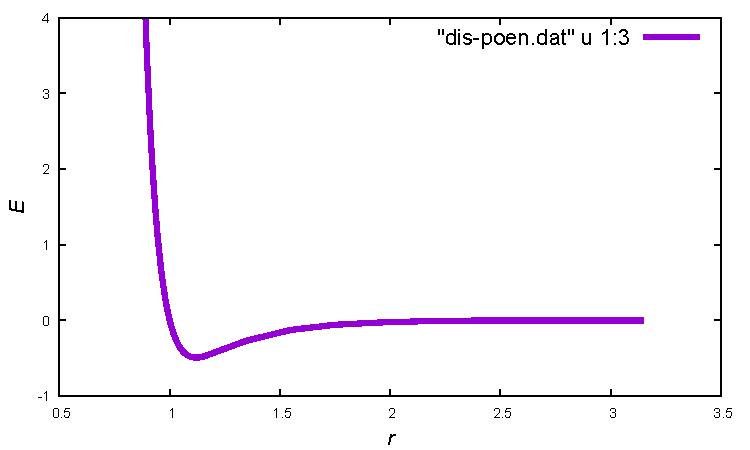
\includegraphics[width=14cm]{fig/dis-poen/dis-poen.pdf}
    \end{center}
    \caption{LJの粒子間距離-ポテンシャルエネルギー。}
    \label{fig:dis-poen}
\end{figure}

% \section{WCAポテンシャル}\label{principle-sec:WCA}
% \ref{principle-sec:LJ}で示したLJポテンシャルの斥力作用と引力作用が入れ替わる$r_c=2^{\frac{1}{6}}{\approx}1.12246$にカットオフ距離を設けたポテンシャルをWCAポテンシャルと呼び、
% WCAポテンシャル粒子系においてもLJ単位系を用いる。
% カットオフ距離とは、その距離内の粒子間の相互作用のみを考慮するものであり、それ以上の距離での粒子間の力を無視するものである\cite{cutoff}。
% WCAポテンシャル粒子系において二つの粒子間相互作用ポテンシャルエネルギーは、
% \large
% \begin{equation}
% \phi(r) = \left\{ \begin{array}{ll}
%     4{\epsilon}\left(\left(\frac{\sigma}{r}\right)^{12}-\left(\frac{\sigma}{r}\right)^6\right) & (r\,{\leq}\,{r_c}) \\
%     0 & (r>r_c)\label{eq:wca}
% \end{array} \right.
% \end{equation}
% \normalsize
% で与えられる\cite{wca}。
% したがって、WCAポテンシャルとはLJポテンシャルの斥力作用と引力作用が入れ替わる$r=r_c$にカットオフ距離を設けることにより、式(\ref{eq:wca})のように二粒子間の引力作用を無視し、斥力作用のみを考慮したポテンシャルである。


% \section{LJ, WCAポテンシャルの比較}\label{principle-sec:LJ-WCA}
% 図\ref{fig:dis-poen}にLJポテンシャル粒子系とWCAポテンシャル粒子系における粒子間距離$r$と粒子間のポテンシャルエネルギー$E$を示す。
% 尚、図\ref{fig:dis-poen}ではLJポテンシャルにカットオフ距離2.5を設けているものとする。

% \newpage
% \begin{figure}[htbp]
%     \begin{center}
%         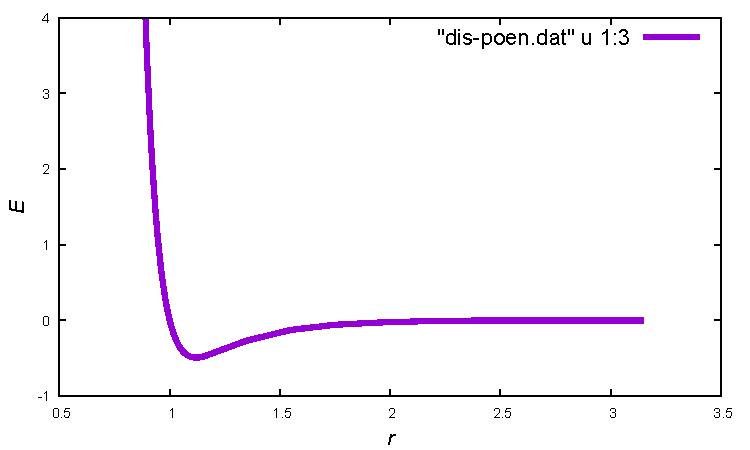
\includegraphics[width=14cm]{fig/dis-poen/dis-poen.pdf}
%     \end{center}
%     \caption{WCAとLJの粒子間距離-ポテンシャルエネルギー。
%     WCAポテンシャルはLJポテンシャルにカットオフ距離$r=r_c$を設けることにより、$r>r_c$でポテンシャルエネルギーが0になっている。}
%     \label{fig:dis-poen}
% \end{figure}

% 図\ref{fig:dis-poen}に示すように、WCAポテンシャルはLJポテンシャルにカットオフ距離$r=r_c$を設けることにより、
% $r>r_c$でポテンシャルエネルギーが0になっている。

\subsection{時間積分}\label{principle-subsec:time-integral}
分子動力学法において、粒子間に働く力を基に粒子を逐次的に動かす手法として速度Verlet法が使用されている。
位置$r(t)$の$t_0$まわりでのテイラー展開は、

\large
\begin{eqnarray}
r(t) &=& r(t_0)+(t-t_0)v(t_0)+\frac{(t-t_0)^2}{2}a(t_0) \label{eq:taylor}
\end{eqnarray}
\normalsize
であることから、$t_0$から微小時間$\Delta{t}$変化した時の位置$r(t+\Delta{t})$は、

\large
\begin{eqnarray}
r(t_0+\Delta{t}) \simeq r(t_0)+\Delta{t}v(t_0)+\frac{\Delta{t}^2}{2}a(t_0) \label{eq:r-renewal-formula}
\end{eqnarray}
\normalsize
で与えられ、これが位置$r(t)$の更新式である\cite{velocity-verlet}。
また、速度$v(t)$は位置の1階微分で求められるので、速度の更新式は

\large
\begin{eqnarray}
v(t_0+\Delta{t}) &=& \frac{d}{dt}r(t_0+\Delta{t}) \nonumber \\
&\simeq& v(t_0)+\frac{\Delta{t}}{2}(a(t_0+\Delta{t})+a(t_0)) \label{eq:v-renewal-formula}
\end{eqnarray}
\normalsize
で与えられる。

\subsection{温度制御}\label{principle-subsec:temperature-control}
$N$粒子系のハミルトニアンは、

\large
\begin{eqnarray}
H(\mathbf{p},\mathbf{r}) &=& \sum_{i=1}^N\frac{\mathbf{p}_i^2}{2m_i}+U(\mathbf{r}_1,...,\mathbf{r}_N) \label{eq:molecular-dynamics-hamiltonian}
\end{eqnarray}
\normalsize
で与えられる\cite{molecular-dynamics-hamiltonian}。ここで、$\mathbf{p}_1,...,\mathbf{p}_N$は粒子の運動量で$\mathbf{p}_i+m_i\mathbf{v}_i$で定義され、$U(\mathbf{r}_1,...,\mathbf{r}_N)$は粒子間のポテンシャルである。
分子動力学法は、与えられたハミルトニアンから導かれるハミルトンの運動方程式を数値積分することで原子の座標や速度を更新していく手法であり、式(\ref{eq:molecular-dynamics-hamiltonian})よりハミルトンの運動方程式は、

\large
\begin{eqnarray}
\dot{\mathbf{r}}_i &=& \frac{\partial H}{\partial \mathbf{p}_i} \label{eq:molecular-dynamics-hamilton-r}
\end{eqnarray}
\normalsize
\large
\begin{eqnarray}
\dot{\mathbf{p}}_i &=& -\frac{\partial H}{\partial \mathbf{r}_i} \label{eq:molecular-dynamics-hamilton-p}
\end{eqnarray}
\normalsize
と書ける。
さらに、式(\ref{eq:molecular-dynamics-hamilton-r}),(\ref{eq:molecular-dynamics-hamilton-p})より、

\large
\begin{eqnarray}
\frac{dH}{dt} &=& \sum_{i=1}^N\Bigg[\frac{\partial H}{\partial \mathbf{r}_i}\dot{\mathbf{r}}_i+\frac{\partial H}{\partial \mathbf{p}_i}\dot{\mathbf{p}}_i\Bigg] \nonumber \\
              &=&  \sum_{i=1}^N\Bigg[\frac{\partial H}{\partial \mathbf{r}_i}\frac{\partial H}{\partial \mathbf{p}_i}i-\frac{\partial H}{\partial \mathbf{p}_i}\frac{\partial H}{\partial \mathbf{r}_i}\Bigg] \nonumber \\
              &=& 0 \label{eq:molecular-dynamics-hamilton-H}
\end{eqnarray}
\normalsize
となるため、単純なMDシミュレーションにおいては全エネルギー$E$が保存され、原子数$N$、体積$V$、エネルギー$E$が一定のNVEアンサンブル\cite{nve-ensemble}が実現される。
ただ、実用的な面で言うとNVEアンサンブルよりも原子数$N$、体積$V$、エネルギー$T$が一定のNVTアンサンブル\cite{nvt-ensemble}が望ましいため、温度制御が必要となる。

温度制御の手法として、速度スケーリング法\cite{velocity-scaling}、ベレンゼン法\cite{berendsen}、能勢フーバー法\cite{nose,hoover}、ランジュバン法\cite{langevin}が存在する。まず、速度スケーリング法は強烈に温度制御をかける手法でシミュレーションとして安定しないため、ベレンゼン法は厳密なカノニカル分布にならない場合があるため、本研究では採用には至らなかった。能勢フーバー法とランジュバン法を比較すると、能勢フーバー法は稀に温度が一様にならない、ランジュバン法は収束が遅い、といった問題点が存在する。
そこで、本研究では温度が一様に制御されることを確認した上で、収束が早く、厳密なカノニカル分布を実現する能勢フーバー法を採用した。
能勢フーバー法は、系が小さい場合でも厳密にカノニカル分布を再現する手法として提案されたもので、能勢フーバー法の運動方程式は、

\large
\begin{eqnarray}
\dot{\mathbf{r}}_i &=& \frac{\partial H}{\partial \mathbf{p}_i} \label{eq:nose-hoover-r}
\end{eqnarray}
\normalsize
\large
\begin{eqnarray}
\dot{\mathbf{p}}_i &=& -\frac{\partial H}{\partial \mathbf{r}_i}-\mathbf{p}_i\zeta \label{eq:nose-hoover-p}
\end{eqnarray}
\normalsize
\large
\begin{eqnarray}
\dot{\zeta} &=& \frac{1}{Q}(T-T_0) \label{eq:nose-hoover-zeta}
\end{eqnarray}
\normalsize
で与えられる。$Q$は熱浴の質量と呼ばれ、緩和の時定数を決める。

ここで、本研究における温度$T$の時間発展を図\ref{fig:time-temperature}に示す。

\begin{figure}[htbp]
    \begin{center}
        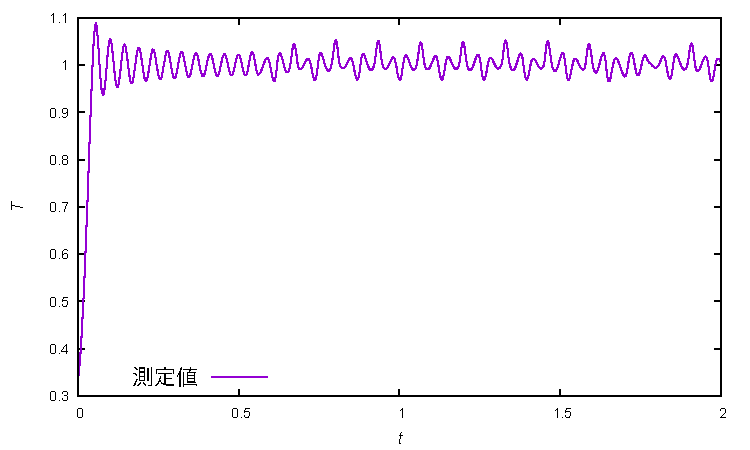
\includegraphics[width=14cm]{fig/nose-hoover/tT.pdf}
    \end{center}
    \caption{温度$T$の時間発展。初期緩和があり、初期緩和後も$T=1.0$の周りで揺らぎが観測される。}
    \label{fig:time-temperature}
\end{figure}

\newpage
図\ref{fig:time-temperature}に示すように、温度$T$は能勢フーバー法により制御されていることが分かる。
初期緩和後も$T=1.0$の周りで揺らぎが見られるが、初期緩和後には、温度$T=1.0$であるとして、解析を行った。


\section{気液共存状態} \label{principle-sec:gas-liquid-coexistence}
共沸現象は気液共存状態が実現され、かつ気相と液相の混合比が等しくなる条件であるから、共沸条件を調べるためには、まず気相と液相の共存状態を達成する必要がある。気液共存状態とは、与えられた環境(温度$T$や圧力$P$)において気相と液相の化学ポテンシャル$\mu$が等しい状況であり、その手法としてGE法、GDI法が用いられてきた。\ref{principle-subsec:gibbs-ensemble}節ではGE法を、\ref{principle-subsec:gibbs-duhem-integration}節ではGDI法をそれぞれ説明する。

\subsection{GE法} \label{principle-subsec:gibbs-ensemble}
ギブスアンサンブルモンテカルロ法(GEMC)は、Panagiotopoulosらによって開発され\cite{gibbs-ensemble-panagiotopoulos-1,gibbs-ensemble-panagiotopoulos-2}、単成分および多成分系の相平衡を効率的に計算するための手法として確立されてきた手法である\cite{gibbs-ensemble-phase-equilibrium-1,gibbs-ensemble-phase-equilibrium-2}。

ギブスアンサンブルモンテカルロ法は、温度$T$で平衡状態にある液体(相A)と気体(相B)をシミュレートするために設計されている\cite{gibbs-ensemble-panagiotopoulos-2}。初期状態として、相Aは体積$V_A$のシミュレーションボックスに$N_A$個の粒子を、相Bは体積$V_B$のシミュレーションボックスに$N_B$個の粒子を含む。尚、粒子の総数$N=N_A+N_B$と総体積$V=V_A+V_B$はシミュレーションにおいて保存されているものとする。これにより二つのシミュレーションボックスは全体として物質量$N$、体積$V$、温度$T$が一定のNVTアンサンブルを形成する。シミュレーションは、粒子配置の変更・体積の再配置・粒子交換で構成される。

\subsubsection{粒子配置の変更}\label{principle-subsubsec:particle-displacement}
このステップでは、各シミュレーションボックスは独立しているものとする。ある粒子がシミュレーションボックスAでランダムに選ばれ、シミュレーションボックスAの新しい位置へ一様なランダム変位が与えられる。この新しい位置への粒子の移動は、$\min(1, \varphi_{move}^A)$の確率で受け入れられる。この$\varphi_{move}^A$は新しい状態と古い状態の確率の比であり、

\large
\begin{eqnarray}
\varphi_{move}^A &=& \exp(-{\beta}E_{new}^A)/\exp(-{\beta}E_{old}^A) \nonumber\\
                 &=& \exp(-{\beta}{\Delta}E^A)\label{eq:particle-displacement-probability}
\end{eqnarray}
\normalsize
で与えられる。尚、${\Delta}E^A$は試行移動のエネルギー変化であり、試行が拒否された場合、マルコフ連鎖の中で古い状態が再集計される。

\subsubsection{体積の再配置}\label{principle-subsubsec:volume-rearrangement}
このステップでは、各シミュレーションボックスでの試行は相関があるものとする。
今、シミュレーションボックスAで$\Delta{V}$体積変化があるとすると、新旧の状態の確率の比は、

\large
\begin{eqnarray}
\varphi_{vol}^A &=& \frac{\exp[-{\beta}P(V^A+{\Delta}V)-{\beta}E^A_{new}+N\ln(V^A+{\Delta}V)]}{\exp[-{\beta}PV^A-{\beta}E^A_{old}+N^A\ln(V^A)]} \nonumber\\
                &=& \exp[-{\beta}P{\Delta}V-{\beta}{\Delta}E^A+N^A\ln(V^A+{\Delta}V)-N^A\ln(V^A)]\label{eq:volume-rearrangement-probability-A}
\end{eqnarray}
\normalsize
で与えられる。
2つのシミュレーションボックスの総体積は保存されているので、シミュレーションボックスBでは${\Delta}V$の体積変化を伴い、等温等圧アンサンブルを満たす系となる。尚、ここでは2つの相が共存する=シミュレーションボックスA,Bの圧力Pは等しいと仮定している。
シミュレーションボックスBの新旧の状態の確率比は、

\large
\begin{eqnarray}
\varphi_{vol}^B &=& \exp[-{\beta}P{\Delta}V-{\beta}{\Delta}E^B+N^B\ln(V^B-{\Delta}V)-N^B\ln(V^B)]\label{eq:volume-rearrangement-probability-B}
\end{eqnarray}
\normalsize
で与えられる。

全体として新旧の状態の確率比は、

\large
\begin{eqnarray}
\varphi_{vol} &=& \varphi_{vol}^A×\varphi_{vol}^B \nonumber
\end{eqnarray}
\normalsize
と書けるので、式(\ref{eq:volume-rearrangement-probability-A}),(\ref{eq:volume-rearrangement-probability-B})より、
\large
\begin{eqnarray}
\varphi_{vol} &=& \exp\Bigg(-\beta\bigg[{\Delta}E^A+{\Delta}E^B-N^{A}kT\ln{\frac{V^A+\Delta{V}}{V^A}}-N^{B}kT\ln{\frac{V^B+\Delta{V}}{V^B}}\bigg]\Bigg) \label{eq:volume-rearrangement-probability-all}
\end{eqnarray}
であり、$\min(1, \varphi_{vol})$の確率で受け入れられる。
試行が拒否された場合、マルコフ連鎖の中で古い状態が再集計される。

\subsubsection{粒子交換}\label{principle-subsubsec:particle-interchange}
このステップでは、各シミュレーションボックスでの試行は相関があるものとする。
今、シミュレーションボックスAで新しい位置がランダムに選ばれる時、新旧の状態の確率の比は、

\large
\begin{eqnarray}
\varphi_{int}^A &=& \frac{\exp[-{\beta}E^A_{new}+\beta(N^A+1)\mu-\ln(N^A+1)!-3(N^A+1)\ln\lambda+(N^A+1)\ln{V^A}]}{\exp[-{\beta}E^A_{old}+{\beta}N^A{\mu}-\ln{N^A!}-3N^A\ln{\lambda}+N^A\ln(V^A)]}  \nonumber\\
                &=& \exp[-{\beta}{\Delta}E^A+\ln(zV^A/(N^A+1))]\label{eq:particle-interchange-probability-A}
\end{eqnarray}
\normalsize
で与えられる。尚、活量係数$z$は、$\exp(\beta\mu)/\lambda^3$で与えられ、$\lambda$は構成粒子のドブロイ波長、$\mu$は化学ポテンシャルである。
2つのシミュレーションボックスの総粒子数は保存されているので、シミュレーションボックスBでは粒子の破壊が試みられ、グランドカノニカルアンサンブルを満たす系となる。尚、ここでは2つの相が共存する=シミュレーションボックスA,Bの化学ポテンシャル$\mu$は等しいと仮定している。
シミュレーションボックスBの新旧の状態の確率比は、

\large
\begin{eqnarray}
\varphi_{int}^B &=& \exp[-{\beta}{\Delta}E^A+\ln(N^B/zV^B)]\label{eq:particle-interchange-probability-B}
\end{eqnarray}
\normalsize
で与えられ、式(\ref{eq:particle-interchange-probability-A}),(\ref{eq:particle-interchange-probability-B})より、全体として新旧の状態の確率比は、

\large
\begin{eqnarray}
\varphi_{int} &=& \varphi_{int}^A×\varphi_{int}^B \nonumber\\
              &=& \exp\Bigg(-\beta\bigg[{\Delta}E^A+{\Delta}E^B+{kT}\ln{\frac{V^B(N^A+1)}{V^AN^B}}\bigg]\Bigg)\label{eq:particle-interchange-probability-all}
\end{eqnarray}
\normalsize
であり、$\min(1, \varphi_{int})$の確率で受け入れられる。
試行が拒否された場合、マルコフ連鎖の中で古い状態が再集計される。


\subsection{GDI法}\label{principle-subsec:gibbs-duhem-integration}
気液共存状態の実現には、相間で示強変数である温度$T$・圧力$P$・化学ポテンシャル$\mu$の一致が必要である。
ギブスアンサンブル法では、示強変数の一致のために粒子の交換が必要であったが、GDI法ではクラウジウス・クラペイロン方程式によって示強変数の一致を実現する。

今、温度$T$、圧力$P$において相Aと相Bの相平衡が実現されているとすると、それぞれの相での化学ポテンシャル$\mu(T,P)$は等しいので、

\large
\begin{eqnarray}
\mu_A(T,P) &=& \mu_B(T,P) \label{eq:gdi-mu}
\end{eqnarray}
\normalsize
が満たされる。
化学ポテンシャルはGibbsの自由エネルギー$G$に等しいので、

\large
\begin{eqnarray}
G_A(T,P) &=& G_B(T,P) \label{eq:gdi-g}
\end{eqnarray}
\normalsize
が満たされ、温度が$T$から$T+\Delta{T}$、平衡圧が$P$から$P+\Delta{P}$になるとすると、

\large
\begin{eqnarray}
G_A(T+\Delta{T},P+\Delta{P}) &=& G_B(T+\Delta{T},P+\Delta{P}) \label{eq:gdi-g-delta}
\end{eqnarray}
\normalsize
が満たされる。
式(\ref{eq:gdi-g-delta})をテイラー展開し、2次以降の微小項を切り捨て、式(\ref{eq:gdi-g})と合わせると、

\large
\begin{eqnarray}
\bigg(\frac{\partial{G_A}}{\partial{T}}\bigg)_PdT + \bigg(\frac{\partial{G_A}}{\partial{P}}\bigg)_TdP &=& \bigg(\frac{\partial{G_B}}{\partial{T}}\bigg)_PdT + \bigg(\frac{\partial{G_B}}{\partial{P}}\bigg)_TdP \label{eq:gdi-partial-g}
\end{eqnarray}
\normalsize
が与えられる。
ここで、ギブスの自由エネルギー$G$はエントロピー$S$、エンタルピー$H$を用いて$G=H-TS$、エンタルピー$H$は気体の内部エネルギー$U$、気体の体積$V$を用いて$H=U+PV$と表されるので

\large
\begin{eqnarray}
dG &=& dH-SdT-TdS \label{eq:gdi-dg}
\end{eqnarray}
\begin{eqnarray}
dH &=& dU+VdP+PdV \label{eq:gdi-dh}
\end{eqnarray}
\normalsize
であり、熱力学第一法則より

\large
\begin{eqnarray}
dU &=& dQ-PdV \nonumber \\
   &=& TdS-PdV \label{eq:thermodynamics}
\end{eqnarray}
\normalsize
であるから、

\large
\begin{eqnarray}
dG &=& dH-SdT-TdS \nonumber\\
   &=& (dU+VdP+PdV)-SdT-TdS \nonumber\\
   &=& {(TdS-PdV)+VdP+PdV}-SdT-TdS \nonumber\\
   &=& VdP-SdT \label{eq:gdi-dg-detail}
\end{eqnarray}
\normalsize
が導かれる。
式(\ref{eq:gdi-dg-detail})において$dT=0$、$dP=0$と仮定すると
\large
\begin{eqnarray}
\bigg(\frac{\partial{G}}{\partial{T}}\bigg)_P &=& -S \label{eq:gdi-dg-dt}
\end{eqnarray}
\begin{eqnarray}
\bigg(\frac{\partial{G}}{\partial{P}}\bigg)_T &=& V \label{eq:gdi-dg-dp}
\end{eqnarray}
\normalsize
であり、式(\ref{eq:gdi-partial-g})にこれを代入すると、

\large
\begin{eqnarray}
-S_AdT+V_AdP &=& -S_BdT+V_BdP \nonumber \\
\Leftrightarrow \frac{dP}{dT} &=& \frac{S_B-S_A}{V_B-V_A} \label{eq:gdi-dp-dt}
\end{eqnarray}
\normalsize
が導かれる。
ここで、$dS=S_B-S_A$は相転移$A\rightarrow{B}$に伴う1molあたりのエントロピー変化であるから、1molあたりの相転移熱を$H$とすると、

\large
\begin{eqnarray}
dS &=& S_B-S_A \nonumber \\
   &=& \frac{\Delta{H}}{T} \label{eq:gdi-ds}
\end{eqnarray}
\normalsize
と表され、式(\ref{eq:gdi-dp-dt}),(\ref{eq:gdi-ds})より、
\large
\begin{eqnarray}
\frac{dP}{dT} &=& \frac{\Delta{H}}{T\Delta{V}} \label{eq:clausius-clapeyron}
\end{eqnarray}
\normalsize
が導かれる。
式(\ref{eq:clausius-clapeyron})がクラウジウス・クラペイロン方程式であり、共存線に沿った温度による圧力の変化を表す方程式である\cite{atkins, clausius-clapeyron1}。


\section{最適化手法}\label{principle-sec:optimization-method}
本研究では、密度のフィッティングにLevenberg-Marquardt(LM)法を用いる。その説明のため、代表的な最適化手法を以下にまとめる。\ref{principle-subsec:least-squares}節では最小二乗法を、\ref{principle-subsec:gradient-descent}節では勾配降下法を、\ref{principle-subsec:gauss-newton}節ではガウス・ニュートン法を、\ref{principle-subsec:levenberg-marquardt}節ではLevenberg-Marquardt法をそれぞれ説明する。

\subsection{最小二乗法}\label{principle-subsec:least-squares}
最小二乗問題は、モデル関数とデータ点の誤差の二乗和で表される目的関数を最小化することで、パラメタ化された数学モデルをデータ点の集合に適合させるものである。今、独立変数$t$と$n$個のパラメタ$\bm{p}$のベクトルからなるモデル関数$\hat{y}(t;\bm{p})$、$m$個のデータ点$(t_i, y_i)$が存在する時、最小二乗問題は$\hat{y}(t;\bm{p})$と$m$個のデータ点$(t_i, y_i)$の間の誤差(または重み付き残差)の重み付き二乗和を最小化することに等しく、目的関数は
\large
\begin{eqnarray}
\chi^2(\bm{p}) &=& \sum_{i=1}^{m}\Bigg[\frac{y(t_i)-\hat{y}(t_i;\bm{p})}{\sigma_(y_i)}\Bigg]^2 \nonumber\\
               &=& (\bm{y}-\hat{\bm{y}}(\bm{p}))^\top\bm{W}(\bm{y}-\hat{\bm{y}}(\bm{p})) \nonumber\\
               &=& \bm{y}^\top\bm{W}\bm{y}-2\bm{y}^\top\bm{W}\hat{\bm{y}}+\hat{\bm{y}}^\top\bm{W}\hat{\bm{y}} \label{eq:queue-residual-error}
\end{eqnarray}
\normalsize
で与えられる。
ここで、$\sigma_(y_i)$はデータ$y(t_i)$の測定誤差、$\bm{W}$は重み付け行列を示す\cite{gradient-descent_gauss-newton_levenberg-marquardt}。

\subsection{勾配降下法}\label{principle-subsec:gradient-descent}
勾配降下法は、パラメタ値を下り坂方向、つまり目的関数の勾配と反対方向に更新する最小化手法である。勾配降下法は、単純な目的関数の最小化問題においては、非常によく収束することが知られている\cite{gradient-descent}。パラメタに関するカイ二乗目的関数の勾配は、
\large
\begin{eqnarray}
\frac{\partial}{\partial\bm{p}}\chi^2 &=& 2(\bm{y}-\hat{\bm{y}}(\bm{p}))^\top\bm{W}\frac{\partial}{\partial\bm{p}}(\bm{y}-\hat{\bm{y}}(\bm{p})) \nonumber\\
                                      &=& -2(\bm{y}-\hat{\bm{y}}(\bm{p}))^\top\bm{W}\Bigg[\frac{\partial\hat{\bm{y}}(\bm{p})}{\partial\bm{p}}\Bigg] \nonumber\\
                                      &=& -2(\bm{y}-\hat{\bm{y}})^\top\bm{W}\bm{J} \label{eq:gradient-of-the-chi-square-objective-function}
\end{eqnarray}
\normalsize
で与えられる。
ここで、$m×n$ヤコビアン行列$\partial\hat{\bm{y}}/{\partial\bm{p}}$は、関数の局所的な感度を表す。
また、パラメタを最急降下の方向に移動させるパラメタ更新$\bm{h}$は、
\large
\begin{eqnarray}
\bm{h} = \alpha\bm{J}^\top\bm{W}(\bm{y}-\hat{\bm{y}})
\end{eqnarray}
\normalsize
で与えられる\cite{gradient-descent_gauss-newton_levenberg-marquardt}。
尚、正のスカラー$\alpha$は、最急降下方向のステップの長さを示す。

\subsection{ガウス・ニュートン法}\label{principle-subsec:gauss-newton}
ガウス。ニュートン法は、最適解の近傍のパラメタにおいて目的関数がほぼ二次関数であることを仮定して\cite{gauss-newton-objective-function}、二乗和の目的関数を最小化する手法である。ガウス・ニュートン法は、適度な大きさの問題では、勾配降下法よりも遥かに速く収束する\cite{gauss-newton}。
摂動されたモデルパラメタで評価される関数は、一次テイラー級数展開により
\large
\begin{eqnarray}
\hat{\bm{y}}(\bm{p}+\bm{h})&\approx&\hat{\bm{y}}(\bm{p})+\Bigg[\frac{\partial\hat{\bm{y}}}{\partial\bm{p}}\bm{h}\Bigg] \nonumber\\
                           &=&\hat{\bm{y}}+\bm{J}\bm{h} \label{gauss-newton_model-parameter}
\end{eqnarray}
\normalsize
と局所的に近似することが出来る。
これを式(\ref{eq:queue-residual-error})に代入すると、
\large
\begin{eqnarray}
\chi^2(\bm{p}+\bm{h}) &\approx& \bm{y}^\top\bm{W}\bm{y}+\bm{y}^\top\bm{W}\hat{\bm{y}}-2\bm{y}^\top\bm{W}\hat{\bm{y}}-2(\bm{y}-\bm{\hat{y}})^\top\bm{W}\bm{J}\bm{h}+\bm{h}^\top\bm{J}^\top\bm{W}\bm{J}\bm{h}
\end{eqnarray}
\normalsize
となり、$\chi^2$を最小にするパラメタ更新$\bm{h}$は、${\partial\chi^2}/{\partial\bm{h}}=0$により、
\large
\begin{eqnarray}
\frac{\partial^2}{\partial\bm{h}}\chi^2(\bm{p}+\bm{h}) &\approx& -2(\bm{y}-\bm{\hat{y}})^\top\bm{W}\bm{J}+2\bm{h}^\top\bm{J}^\top\bm{W}\bm{J}
\end{eqnarray}
\normalsize
で与えられる。
以上より、ガウス・ニュートン更新のための正規方程式は、
\large
\begin{eqnarray}
\Big[\bm{J}^\top\bm{W}\bm{J}\Big]\bm{h} = \bm{J}^\top\bm{W}(\bm{y}-\bm{\hat{y}})
\end{eqnarray}
\normalsize
で与えられる\cite{gradient-descent_gauss-newton_levenberg-marquardt}。

\subsection{Levenberg-Marquardrt法}\label{principle-subsec:levenberg-marquardt}
Lebenberg-Marquardrt法は、非線形最小二乗問題を解くために1960年代初頭に開発された最適化アルゴリズムであり、様々な問題において、単純な勾配降下法や他の共役勾配法よりも大幅に優れていることが知られている\cite{levenberg-marquardt}。
勾配降下法では、最急降下方向にパラメタを更新することにより、二乗誤差の和を減少させる。ガウス・ニュートン法では、最小二乗関数は局所的に二次関数であると仮定して、二乗誤差の総和を小さくする。
Levenberg-Marquardtアルゴリズムは、勾配降下法とガウス・ニュートン法という2つの数値的最小化アルゴリズムを組み合わせたもので、パラメタ更新式は、
\large
\begin{eqnarray}
\Big[\bm{J}^\top\bm{W}\bm{J}+\lambda\bm{I}\Big]\bm{h} = \bm{J}^\top\bm{W}(\bm{y}-\bm{\hat{y}})
\end{eqnarray}
\normalsize
と表せ、Levenberg-Marquardt法は、パラメタが最適値から遠い($\lambda$の値が大きい)場合は勾配降下更新をし、パラメタが最適値に近い($\lambda$の値が小さい)場合はガウス・ニュートン更新をする\cite{gradient-descent_gauss-newton_levenberg-marquardt}。


\chapter{手法} \label{chap:method}
\ref{method-sec:mono-component}節では、単成分LJ系における気液共存状態の実現手法を述べる。
\ref{method-sec:bi-component-azeotrope}節では、二成分LJ系における共沸現象の実現手法を述べる。
\ref{method-sec:bi-component-potential-parameter-azeotrope-ratio}節では、二成分LJ系におけるポテンシャルパラメタと共沸組成の関係の推定手法を述べる。
\ref{method-sec:bi-component-addition-of-3rd-component-highest-purity}節では、二成分LJ系への第三成分の添加手法と添加による目的物質の最高濃度の上昇を確認する手法を述べる。
\ref{method-sec:bi-component-addition-of-3rd-component-steps}節では、二成分LJ系への第三成分の添加手法と添加による特定段数で到達する目的物質の濃度の上昇を確認する手法を述べる。


\section{単成分LJ系における気液共存状態の実現} \label{method-sec:mono-component}
LJ系では、ある温度、密度条件では気相と液相が相分離することが平衡状態(=気液共存状態)である事が知られている\cite{gas-liquid-equilibrium}。本節では、実際にMDシミュレーションによりこの事実を観測し、条件の近い先行研究と比較し大きな相違がないことを確認する。
初期状態として$100×50×50$の直方体の左半分に$N=78732(27×27×27×4)$個の粒子を、右半分に$N=10976(14×14×14×4)$個の粒子を面心立方(face-centered cubic, fcc)構造上に配置する。図\ref{fig:ln78732-rn10976-ld0.629856-rd0.087808-first}に、粒子の初期配置を示す。

\begin{figure}[htbp]
    \begin{center}
        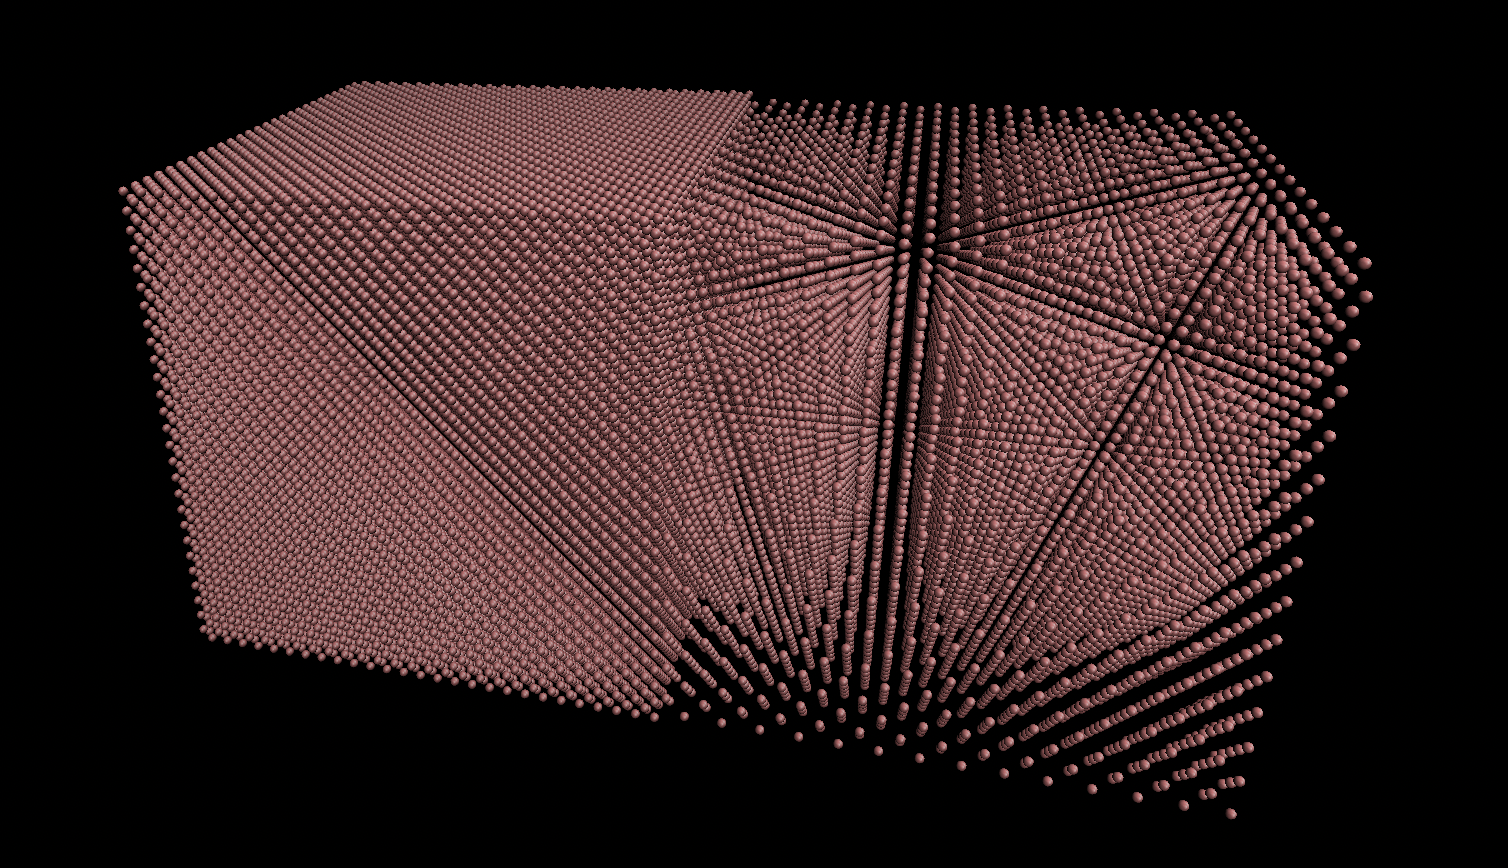
\includegraphics[width=14cm]{fig/ln78732-rn10976-ld0.629856-rd0.087808/ln78732-rn10976-ld0.629856-rd0.087808-first.png}
    \end{center}
    \caption{単成分LJ系のMDシミュレーションにおける粒子の初期配置。fcc構造上に配置されている。}
    \label{fig:ln78732-rn10976-ld0.629856-rd0.087808-first}
\end{figure}

\newpage
この初期配置の下、実行したシミュレーションにおけるパラメタを表\ref{table:mono-component-parameter}に、粒子間のポテンシャルパラメタ及びカットオフ距離を表\ref{table:mono-component-potential-parameter}に示す。

\begin{table}[htbp]
    \begin{center}
        \caption{各パラメタの値}
        \label{table:mono-component-parameter}
            \begin{tabular}{c c c}
                $T$ & timestep & ステップ数 \\
                \hline
                1.0 & 0.001 & 505000 \\
            \end{tabular}
    \end{center}
\end{table}

\begin{table}[htbp]
    \begin{center}
        \caption{各ポテンシャルパラメタ及びカットオフ距離の値}
        \label{table:mono-component-potential-parameter}
            \begin{tabular}{c c c}
                $\sigma$ & $\epsilon$ & $r_c$ \\
                \hline
                1.0 & 1.0 & 3.0\\
            \end{tabular}
    \end{center}
\end{table}

表\ref{table:mono-component-parameter}, \ref{table:mono-component-potential-parameter}に示したパラメタを基に、MDシミュレーションをLAMMPSで実行して、粒子の座標を出力し、各位置$x$\,(0.0〜1.0の0.001刻み)における密度を測定する。尚、粒子の密度は最後の5000ステップから1000ステップ刻みに各粒子の位置座標を出力した5個の結果の平均を取るものとする。このように粒子の密度を測定しプロットすることで、最終的に気液共存状態が実現されていることを確認する。
\ref{results-sec:mono-component}節では、このシミュレーション実行時の粒子の密度の測定, 気液共存状態が実現されていることの確認および、条件の近い先行研究との密度の比較を行う。


\section{二成分LJ系における共沸現象の実現} \label{method-sec:bi-component-azeotrope}
共沸現象とは液体混合物が沸騰する際に気相と液相の組成が等しくなる現象を指す。ここで、液体混合物が沸騰する温度のことを沸点と呼ぶが、沸点とは液体の飽和蒸気圧が外圧と等しくなる温度のことを指し\cite{atkins}、この温度において一定圧力の元で飽和蒸気とその液体とが平衡を保って共存する。このことから、共沸現象とは気液共存状態において液体混合物の気相と液相の組成が同じになる現象のことを指し、二成分(以降では、二成分をA, Bとする)の気液共存状態におけるA, Bの気相密度を$g_A, g_B$、液相密度を$l_A, l_B$とすると、共沸条件はそれぞれの成分において気相と液相の密度比が等しくなることであるから$X=g_Al_B-l_Ag_B$と定義すると共沸点は$X=0$で与えられる(以降では、$X$を共沸パラメタと呼ぶ)。

シミュレーションは、初期状態として$200×100×100$の直方体の左半分にA, B合わせて$N=702464(56×56×56×4)$個の粒子を、右半分に$N=19652(17×17×17×4)$個の粒子を面心立方(face-centered cubic, fcc)構造上に配置する。図\ref{fig:lan140493-lbn561971-ran3930-rbn15722-first}に、Aの組成比0.2, Bの組成比0.8の時の粒子の初期配置を示す。

\begin{figure}[htbp]
    \begin{center}
        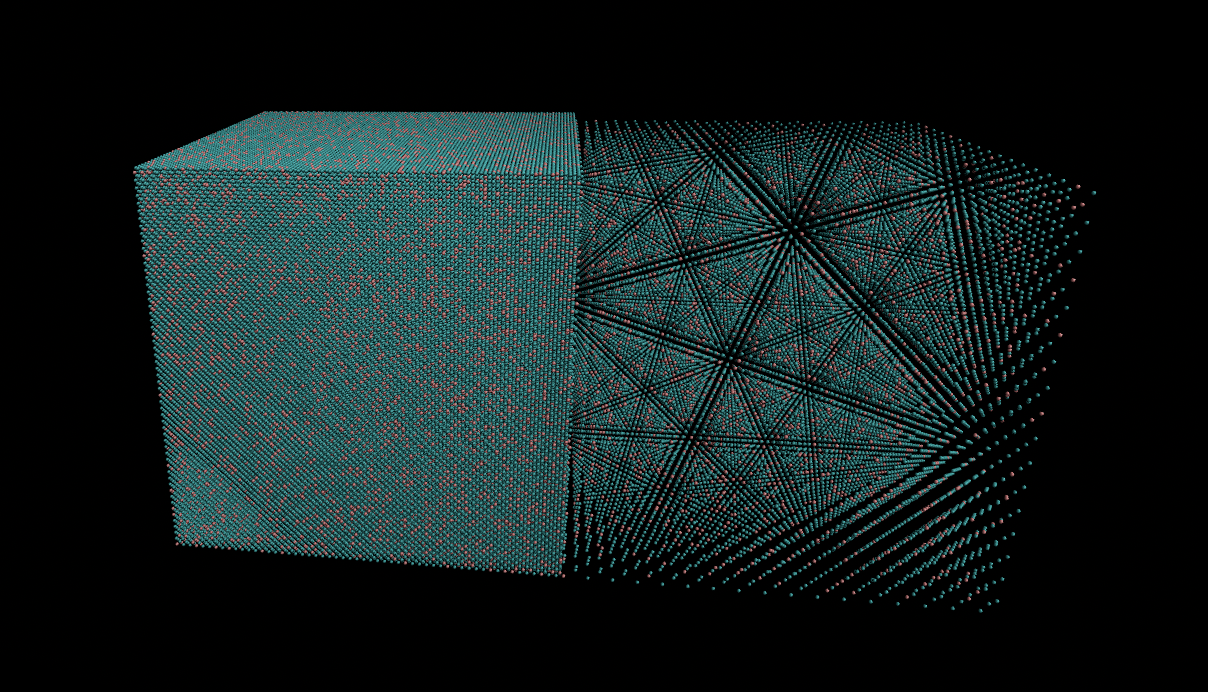
\includegraphics[width=14cm]{fig/lan140493-lbn561971-ran3930-rbn15722/lan140493-lbn561971-ran3930-rbn15722-first.png}
    \end{center}
    \caption{二成分LJ系のMDシミュレーションにおける粒子の初期配置。fcc構造上に配置されている。
    桃色が粒子A, 水色が粒子Bを指す。}
    \label{fig:lan140493-lbn561971-ran3930-rbn15722-first}
\end{figure}

この初期配置の下、相互作用が対称な二成分LJ系と非対称な二成分LJ系においてシミュレーションを行う。尚、以降の研究では、主要な計算資源として東京大学物性研究所の共同利用スーパーコンピュータ ohtaka を用いた。ohtakaは、1ノードに128コアをもつAMD Romeを搭載した標準的な構成のCPUノードと1ノードあたり3TBの大容量メモリを搭載したFatノードで構成されるスーパーコンピューターである\cite{ohtaka}。
まず、CPUノードは1680ノード(420筐体/24ラック)存在し、1ノードあたり4.096TFLOPS(2.0GHz×64core×16命令×2sock)の理論演算性能、409.6GByte/sec(3,200MHz×16channel×8Byte)のメモリ転送性能を誇り、1ノードあたり128コア、1コアあたり2GBのメモリ容量を持つ。
続いて、Fatノードは8ノード存在し、1ノードあたり9.6768TFLOPS(2.7GHz×28core×32命令×4sock)の理論演算性能、563.136GByte/sec(2,933MHzx24channelx8Byte)のメモリ転送性能を誇り、1ノードあたり112コア、1コアあたり約27GBのメモリ容量を持つ。

\subsection{相互作用が対称な二成分LJ系における共沸現象の実現} \label{method-subsec:bi-symmetric-component-azeotrope}
相互作用が対称な二成分LJ系において実行したシミュレーションにおけるパラメタを表\ref{table:symmetric-bi-component-azeotrope-parameter}に、各粒子間のポテンシャルパラメタ及びカットオフ距離を表\ref{table:symmetric-bi-component-azeotrope-potential-parameter}に示す。

\begin{table}[htbp]
    \begin{center}
        \caption{各パラメタの値}
        \label{table:symmetric-bi-component-azeotrope-parameter}
            \begin{tabular}{c c c}
                $T$ & timestep & ステップ数 \\
                \hline
                1.0 & 0.001 & 4000000 \\
            \end{tabular}
    \end{center}
\end{table}

\begin{table}[htbp]
    \begin{center}
        \caption{各ポテンシャルパラメタ及びカットオフ距離の値}
        \label{table:symmetric-bi-component-azeotrope-potential-parameter}
            \begin{tabular}{c c c c}
                & $\sigma$ & $\epsilon$ & $r_c$ \\
                \hline
                A-A & 1.0 & 1.0 & 3.0 \\
                A-B & 1.05 & 0.9 & 3.0 \\
                B-B & 1.0 & 1.0 & 3.0
            \end{tabular}
    \end{center}
\end{table}

\newpage
表\ref{table:symmetric-bi-component-azeotrope-parameter}, \ref{table:symmetric-bi-component-azeotrope-potential-parameter}に示したパラメタを基に、MDシミュレーションをLAMMPSで実行して、各粒子の座標を出力し、各位置$x$\,(0.0〜1.0の0.0025刻み)における密度を測定する。尚、各粒子の密度は最後の1000000ステップから1000ステップ刻みに各粒子の位置座標を出力した1000個の結果の平均を取るものとする。このように粒子の密度を測定しプロットすることで、最終的に気液共存状態が実現されていることを確認する。

\ref{results-subsec:bi-symmetric-component-azeotrope}節では、Aの組成比を0.02〜0.98に0.02刻みで変化させ、各組成比において上記の手法で気液共存状態を実現する。その後、気液共存状態におけるA, Bの気相密度$g_A, g_B$、液相密度$l_A, l_B$を元に各組成比において共沸パラメタ$X=g_Al_B-l_Ag_B$を求め、共沸パラメタ$X=0$となる共沸組成を導出する。尚、本研究ではAの組成比を0.02〜0.98に0.02刻みで変化させた49本のシミュレーションを1つのジョブでスーパーコンピュータohtakaで並列実行した。また、1本のシミュレーションあたり2ノード、256プロセス並列、1スレッド並列で実行した。


\subsection{相互作用が非対称な二成分LJ系における共沸現象の実現} \label{method-subsec:bi-asymmetric-component-azeotrope}
相互作用が非対称な二成分LJ系において実行したシミュレーションにおけるパラメタを表\ref{table:asymmetric-bi-component-azeotrope-parameter}に、各粒子間のポテンシャルパラメタ及びカットオフ距離を表\ref{table:asymmetric-bi-component-azeotrope-potential-parameter}に示す。

\begin{table}[htbp]
    \begin{center}
        \caption{各パラメタの値}
        \label{table:asymmetric-bi-component-azeotrope-parameter}
            \begin{tabular}{c c c}
                $T$ & timestep & ステップ数 \\
                \hline
                1.0 & 0.001 & 4000000 \\
            \end{tabular}
    \end{center}
\end{table}

\begin{table}[htbp]
    \begin{center}
        \caption{各ポテンシャルパラメタ及びカットオフ距離の値}
        \label{table:asymmetric-bi-component-azeotrope-potential-parameter}
            \begin{tabular}{c c c c}
                & $\sigma$ & $\epsilon$ & $r_c$ \\
                \hline
                A-A & 1.0 & 1.0 & 3.0 \\
                A-B & 1.05 & 0.9 & 3.0 \\
                B-B & 1.0 & 1.05 & 3.0
            \end{tabular}
    \end{center}
\end{table}

表\ref{table:asymmetric-bi-component-azeotrope-parameter}, \ref{table:asymmetric-bi-component-azeotrope-potential-parameter}パラメタを基に、MDシミュレーションをLAMMPSで実行して、各粒子の座標を出力し、各位置$x$\,(0.0〜1.0の0.0025刻み)における密度を測定する。尚、各粒子の密度は最後の1000000ステップから1000ステップ刻みに各粒子の位置座標を出力した1000個の結果の平均を取るものとする。このように粒子の密度を測定しプロットすることで、最終的に気液共存状態が実現されていることを確認する。

\ref{results-subsec:bi-asymmetric-component-azeotrope}節では、Aの組成比を0.02〜0.98に0.02刻みで変化させ、各組成比において上記の手法で気液共存状態を実現する。その後、気液共存状態におけるA, Bの気相密度$g_A, g_B$、液相密度$l_A, l_B$を元に各組成比において共沸パラメタ$X=g_Al_B-l_Ag_B$を求め、共沸パラメタ$X=0$となる共沸組成を導出する。尚、本研究ではAの組成比を0.02〜0.98に0.02刻みで変化させた49本のシミュレーションを1つのジョブでスーパーコンピュータohtakaで並列実行した。また、1本のシミュレーションあたり2ノード、256プロセス並列、1スレッド並列で実行した。


\section{二成分LJ系におけるポテンシャルパラメタと共沸組成の関係} \label{method-sec:bi-component-potential-parameter-azeotrope-ratio}
手法\ref{method-sec:bi-component-azeotrope}で観測した共沸現象の内、非対称LJ系に着目する。本研究で採用した、LJポテンシャルは、ポテンシャルパラメタとして、${\sigma}$,\,${\epsilon}$の二つのパラメタが存在する。
本節では、この二つのパラメタを変化させた時の共沸組成の変化を観測する。


\subsection{二成分LJ系における$\sigma$と共沸組成の関係} \label{method-subsec:bi-component-sigma-azeotrope-ratio}
二成分LJ系において${\sigma}$を変化させた時のシミュレーションにおけるパラメタを表\ref{table:bi-component-sigma-azeotrope-ratio-parameter}に、各粒子間のポテンシャルパラメタ及びカットオフ距離を表\ref{table:bi-component-sigma-azeotrope-ratio-potential-parameter}に示す。

\begin{table}[htbp]
    \begin{center}
        \caption{各パラメタの値}
        \label{table:bi-component-sigma-azeotrope-ratio-parameter}
        \begin{tabular}{c c c}
            $T$ & timestep & ステップ数 \\
            \hline
            1.0 & 0.001 & 4000000 \\
        \end{tabular}
    \end{center}
\end{table}

\begin{table}[htbp]
    \begin{center}
        \caption{各ポテンシャルパラメタ及びカットオフ距離の値}
        \label{table:bi-component-sigma-azeotrope-ratio-potential-parameter}
        \begin{tabular}{c c c c}
            & $\sigma$ & $\epsilon$ & $r_c$ \\
            \hline
            A-A & 1.0 & 1.0 & 3.0 \\
            A-B & 1.05 & 0.9 & 3.0 \\
            B-B & variable & 1.0 & 3.0
        \end{tabular}
    \end{center}
\end{table}

\ref{results-subsec:bi-component-sigma-azeotrope-ratio}節では、上記のパラメタを元にシミュレーションを行い、各$\sigma$において\ref{method-subsec:bi-asymmetric-component-azeotrope}節と同様な手法で共沸組成を求め、$\sigma$と共沸組成の関係を導出する。


\subsection{二成分LJ系における$\epsilon$と共沸組成の関係} \label{method-subsec:bi-component-epsilon-azeotrope-ratio}
二成分LJ系において${\epsilon}$を変化させた時のシミュレーションにおけるパラメタを表\ref{table:bi-component-epsilon-azeotrope-ratio-parameter}に、各粒子間のポテンシャルパラメタ及びカットオフ距離を表\ref{table:bi-component-epsilon-azeotrope-ratio-potential-parameter}に示す。

\begin{table}[htbp]
    \begin{center}
        \caption{各パラメタの値}
        \label{table:bi-component-epsilon-azeotrope-ratio-parameter}
        \begin{tabular}{c c c}
            $T$ & timestep & ステップ数 \\
            \hline
            1.0 & 0.001 & 4000000 \\
        \end{tabular}
    \end{center}
\end{table}

\begin{table}[htbp]
    \begin{center}
        \caption{各ポテンシャルパラメタ及びカットオフ距離の値}
        \label{table:bi-component-epsilon-azeotrope-ratio-potential-parameter}
        \begin{tabular}{c c c c}
            & $\sigma$ & $\epsilon$ & $r_c$ \\
            \hline
            A-A & 1.0 & 1.0 & 3.0 \\
            A-B & 1.05 & 0.9 & 3.0 \\
            B-B & 1.0 & variable & 3.0
        \end{tabular}
    \end{center}
\end{table}

\newpage
\ref{results-subsec:bi-component-epsilon-azeotrope-ratio}節では、上記のパラメタを元にシミュレーションを行い、各$\epsilon$において\ref{method-subsec:bi-asymmetric-component-azeotrope}節と同様な手法で共沸組成を求め、$\epsilon$と共沸組成の関係を導出する。


\section{相互作用が対称な二成分LJ系への第三成分の添加による目的物質の最高濃度の上昇} \label{method-sec:bi-component-addition-of-3rd-component-highest-purity}
\subsection{第三成分の添加による目的物質の最高濃度の上昇} \label{method-subsec:bi-component-addition-of-3rd-component-highest-purity}
蒸留によって得られる目的物質の最高濃度は共沸現象によって頭打ちになるが、第三成分を添加することにより、共沸混合物の組成を変化させ、目的物質の最高濃度を上げることが出来る\cite{azeotrope-add_third_component}。本節では、相互作用が対称な二成分LJ系(A, Bとする)に第三成分(Cとする)を添加するシミュレーションによって、共沸組成が変化することで目的物質の最高濃度が上がることを確認する。

シミュレーションは、初期状態として$200×100×100$の直方体の左半分にA, B, C合わせて$N=702464(56×56×56×4)$個の粒子を、右半分に$N=19652(17×17×17×4)$個の粒子を面心立方(face-centered cubic, fcc)構造上に配置する。尚、シミュレーションではCの組成比を0.01(添加割合$1.0\%$)で固定して、Aの組成比を0.0198〜0.9702に0.0198刻みで変化させて、それぞれの粒子をランダムに配置する。図\ref{fig:lan139088-lbn556351-lcn7025-ran3891-rbn15564-rcn197-first}に、Aの組成比0.396, Bの組成比0.594, Cの組成比0.01の時の粒子の初期配置を示す。

\begin{figure}[htbp]
    \begin{center}
        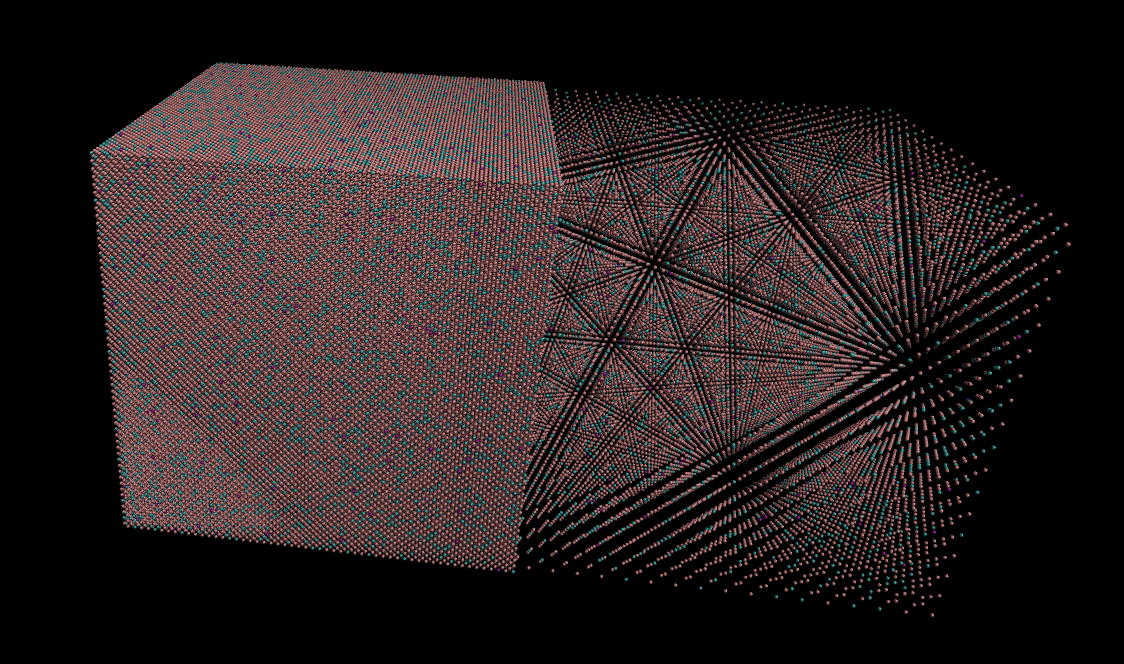
\includegraphics[width=14cm]{fig/lan278176-lbn417263-lcn7025-ran7782-rbn11673-rcn197/lan139088-lbn556351-lcn7025-ran3891-rbn15564-rcn197-first.png}
    \end{center}
    \caption{二成分LJ系のMDシミュレーションにおける粒子の初期配置。fcc構造上に配置されている。水色が粒子A, 桃色が粒子B, 紫色が粒子Cを指す。}
    \label{fig:lan139088-lbn556351-lcn7025-ran3891-rbn15564-rcn197-first}
\end{figure}

\newpage
この初期配置の下、実行したシミュレーションにおけるパラメタを表\ref{table:bi-component-addition-of-3rd-component-parameter}に、粒子間のポテンシャルパラメタ及びカットオフ距離を表\ref{table:bi-component-addition-of-3rd-component-potential-parameter}に示す。

\begin{table}[htbp]
    \begin{center}
        \caption{各パラメタの値}
        \label{table:bi-component-addition-of-3rd-component-parameter}
        \begin{tabular}{c c c}
            $T$ & timestep & ステップ数 \\
            \hline
            1.0 & 0.001 & 7000000 \\
        \end{tabular}
    \end{center}
\end{table}

\begin{table}[htbp]
    \begin{center}
        \caption{各ポテンシャルパラメタ及びカットオフ距離の値}
        \label{table:bi-component-addition-of-3rd-component-potential-parameter}
        \begin{tabular}{c c c c}
            & $\sigma$ & $\epsilon$ & $r_c$ \\
            \hline
            A-A & 1.0 & 1.0 & 3.0 \\
            A-B & 1.05 & 0.9 & 3.0 \\
            B-B & 1.0 & 1.0 & 3.0 \\
            A-C & 1.0 & 2.0 & 3.0 \\
            B-C & 1.0 & 1.0 & 3.0 \\
            C-C & 1.0 & 2.0 & 3.0
        \end{tabular}
    \end{center}
\end{table}

表\ref{table:bi-component-addition-of-3rd-component-potential-parameter}に示したように、第三成分CはAとは強い引力相互作用をもち、Bとは弱い引力相互作用を持つ。

\ref{results-subsec:bi-component-addition-of-3rd-component-highest-purity}節では、上記のパラメタを元にシミュレーションを行い、相互作用が対称な二成分LJ系の結果(\ref{results-subsec:bi-symmetric-component-azeotrope}節)の共沸組成と比較し、共沸組成が変化し目的物質(=B)の最高濃度が上がることを確認する。尚、本研究ではAの組成比を0.0198〜0.9702に0.0198刻みで変化させた49本のシミュレーションを1つのジョブでスーパーコンピュータohtakaで並列実行した。また、1本のシミュレーションあたり2ノード、256プロセス並列、1スレッド並列で実行した。


\subsection{第三成分の添加割合と目的物質の最高濃度の関係} \label{method-subsec:bi-component-addition-of-3rd-component-addition-ratio-highest-purity}
本節では、第三成分Cの添加割合のみを変化させ、\ref{method-subsec:bi-component-addition-of-3rd-component-highest-purity}節と同様のシミュレーションを行う。

\ref{results-subsec:bi-component-addition-of-3rd-component-addition-ratio-highest-purity}節では、Cの添加割合を$0.0,0.5,1.0,1.5,2.0\%$で変化させたときのCの添加割合と目的物質Bの最高濃度の関係を観測する。


\section{相互作用が対称な二成分LJ系への第三成分の添加による特定段数で到達する目的物質の濃度の上昇} \label{method-sec:bi-component-addition-of-3rd-component-steps}
\subsection{第三成分の添加による特定段数で到達する目的物質の濃度の上昇} \label{method-subsec:bi-component-addition-of-3rd-component-steps}
蒸留においては、目的物質の最高濃度に達するまでの段数も重要となるが、これも第三成分を添加することにより減らすことが出来る\cite{distillation}。
本節では、相互作用が対称な二成分LJ系(A, Bとする)に第三成分(Cとする)を添加するシミュレーションによって、特定段数で到達する目的物質の濃度が上がることを確認する。
ただし、本節のシミュレーション条件は、\ref{method-subsec:bi-component-addition-of-3rd-component-highest-purity}節で示したものと同様であるとする。

\ref{results-subsec:bi-component-addition-of-3rd-component-steps}節では、目的物質Bの初期濃度0.1の時、相互作用が対称な二成分LJ系(\ref{results-subsec:bi-symmetric-component-azeotrope}節)において三段で到達する濃度と、第三成分を添加した系において三段で到達する濃度を比較し、第三成分を添加することによって目的物質Bの濃度が上がることを確認する。


\subsection{第三成分の添加割合と特定段数で到達する目的物質の濃度の関係} \label{method-subsec:bi-component-addition-of-3rd-component-addition-ratio-steps}
本節では、第三成分Cの添加割合のみを変化させた上で\ref{method-subsec:bi-component-addition-of-3rd-component-steps}節と同様のシミュレーションを行う。

\ref{results-subsec:bi-component-addition-of-3rd-component-addition-ratio-steps}節では、Cの添加割合を$0.0,0.5,1.0,1.5,2.0\%$で変化させたときの第三成分の添加割合と三段で到達する目的物質Bの濃度の関係を観測する。


\chapter{結果} \label{chap:results}
\ref{results-sec:mono-component}節では、単成分LJ系において気液共存状態を実現する。
\ref{results-sec:bi-component-azeotrope}節では、二成分LJ系において共沸現象を実現する。
\ref{results-sec:bi-component-potential-parameter-azeotrope-ratio}節では、二成分LJ系におけるポテンシャルパラメタと共沸組成の関係を示す。
\ref{results-sec:bi-component-addition-of-3rd-component-highest-purity}節では、二成分LJ系への第三成分の添加による共沸組成のずれ、及び目的物質の最高濃度の上昇を観測する。
\ref{results-sec:bi-component-addition-of-3rd-component-steps}節では、二成分LJ系への第三成分の添加による特定段数で到達する目的物質の濃度の上昇を観測する。

\section{単成分LJ系における気液共存状態の実現} \label{results-sec:mono-component}
\ref{method-sec:mono-component}節で示したパラメタでMDシミュレーションをLAMMPSで実行して、各粒子の座標を出力する。図\ref{fig:ln78732-rn10976-ld0.629856-rd0.087808-last}に、最終ステップの粒子のスナップショットを示す。
\begin{figure}[htbp]
    \begin{center}
        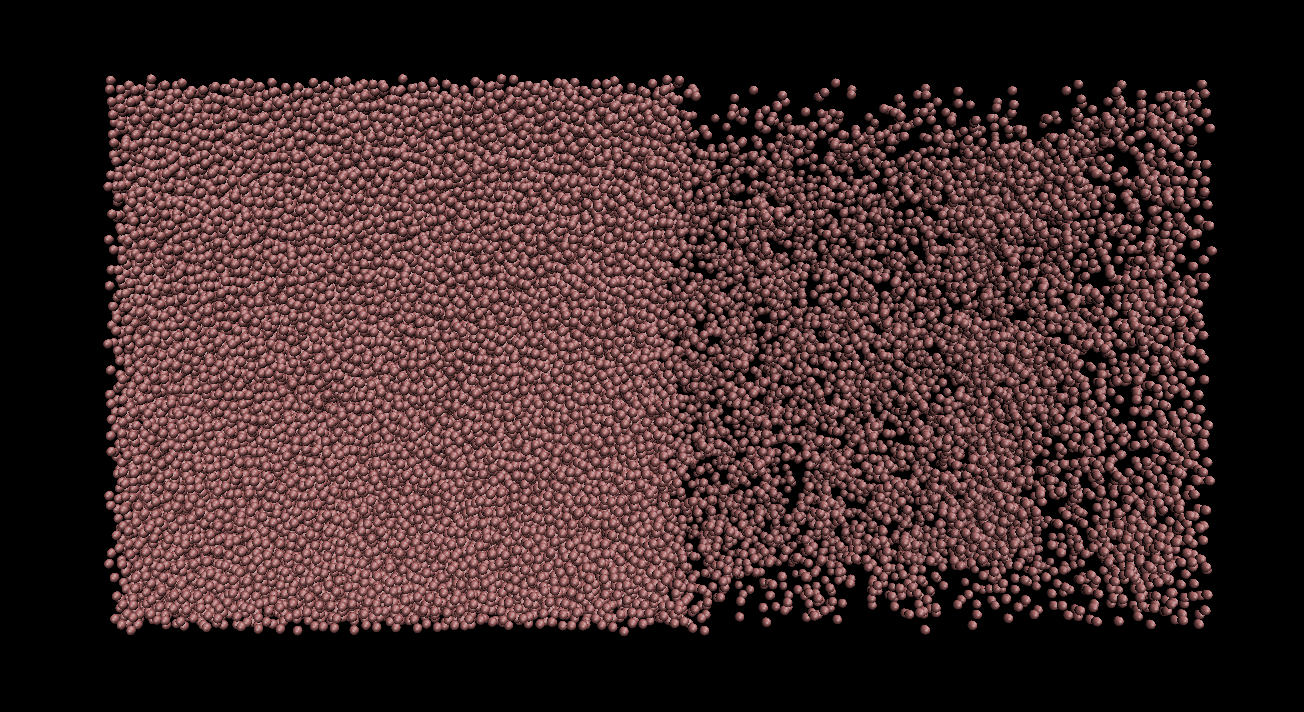
\includegraphics[width=14cm]{fig/ln78732-rn10976-ld0.629856-rd0.087808/ln78732-rn10976-ld0.629856-rd0.087808-last.png}
    \end{center}
    \caption{単成分LJ系のMDシミュレーションにおける最終ステップの粒子のスナップショット。}
    \label{fig:ln78732-rn10976-ld0.629856-rd0.087808-last}
\end{figure}

図\ref{fig:ln78732-rn10976-ld0.629856-rd0.087808-last}の出力結果を元に測定された、各位置$x$\,(0.0:最小、1.0:最大において0.2〜0.8の範囲)とその密度の関係を図\ref{fig:ln78732-rn10976-ld0.629856-rd0.087808}に示す。ただし、密度は、最後の5ステップを平均して取得するものとする。

\begin{figure}[htbp]
    \begin{center}
        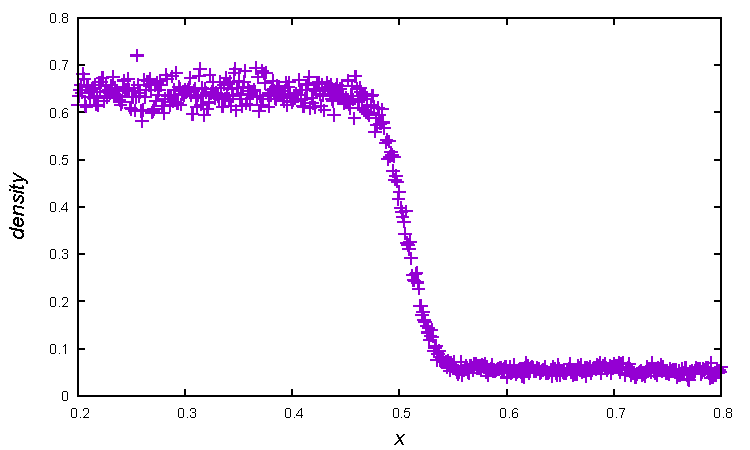
\includegraphics[width=14cm]{fig/ln78732-rn10976-ld0.629856-rd0.087808/ln78732-rn10976-ld0.629856-rd0.087808.pdf}
    \end{center}
    \caption{単成分LJ系における密度の位置依存性}
    \label{fig:ln78732-rn10976-ld0.629856-rd0.087808}
\end{figure}

図\ref{fig:ln78732-rn10976-ld0.629856-rd0.087808}より、$x:0.2〜0.45$で液体状態を、$x:0.45〜0.55$で気液界面を、$x:0.55〜0.8$で気体状態をとる、気液共存状態が実現されていることが分かる。ここで、気液界面およびその近傍の密度プロファイルの関数は、次のような式で表されることが知られている\cite{gas-liquid-interface-density-profile}。
\large
\begin{eqnarray}
    \rho(x) = \frac{\rho_l+\rho_g}{2} - \frac{\rho_l-\rho_g}{2}\,\tanh\Bigg(\frac{x-x_d}{2\delta_d}\Bigg) \label{eq:gas-liquid-interface-density-profile}
\end{eqnarray}
\normalsize
ここで、$\rho_l$は液相密度、$\rho_g$は気相密度、$x_d$は分割面の位置、$\delta_d$は界面厚さを示す。

図\ref{fig:ln78732-rn10976-ld0.629856-rd0.087808}で得られた密度を式(\ref{eq:gas-liquid-interface-density-profile})を目的関数としLevenberg-Marquardt法により近似したものを図\ref{fig:ln78732-rn10976-ld0.629856-rd0.087808-fitting}に示す。

\begin{figure}[htbp]
    \begin{center}
        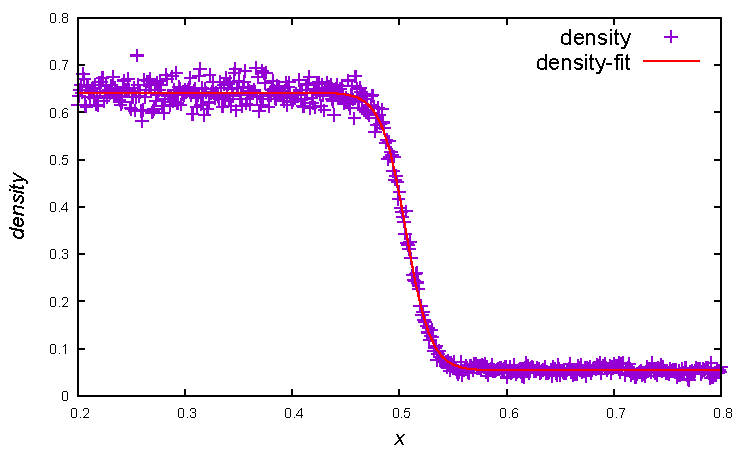
\includegraphics[width=14cm]{fig/ln78732-rn10976-ld0.629856-rd0.087808/ln78732-rn10976-ld0.629856-rd0.087808-fitting.pdf}
    \end{center}
    \caption{単成分LJ系における密度の位置依存性及びその近似}
    \label{fig:ln78732-rn10976-ld0.629856-rd0.087808-fitting}
\end{figure}

\newpage
続いて、表\ref{table:ln78732-rn10976-ld0.629856-rd0.087808-fitting}に、先行研究\cite{gas-liquid-equilibrium}における気液密度と、図\ref{fig:ln78732-rn10976-ld0.629856-rd0.087808-fitting}の近似で得られた気液密度を示す。

\begin{table}[htbp]
    \begin{center}
        \caption{単成分LJ系における密度近似による気液密度値}
        \label{table:ln78732-rn10976-ld0.629856-rd0.087808-fitting}
            \begin{tabular}{c || c | c}
                & $\rho_l$ & $\rho_g$ \\
                先行研究 & 0.5891(1) & 0.0856(2) \\
                本研究 & 0.641(1) & 0.054(1)
            \end{tabular}
    \end{center}
\end{table}

表\ref{table:ln78732-rn10976-ld0.629856-rd0.087808-fitting}より、本研究と先行研究には誤差が存在するが、これは本研究と先行研究とでカットオフ距離近傍での粒子間相互作用がわずかに違うため生じたものと考えられる。そのため、本研究で得られた結果は妥当であると判断し、表\ref{table:ln78732-rn10976-ld0.629856-rd0.087808-fitting}で得た平衡状態における気液密度を基に、以降では初期状態で凡その気体状態、液体状態を実現した上で研究を進めることにより、平衡状態までの収束を早めた。


\section{二成分LJ系における共沸現象の実現} \label{results-sec:bi-component-azeotrope}
\subsection{相互作用が対称な二成分LJ系における共沸現象の実現} \label{results-subsec:bi-symmetric-component-azeotrope}
\ref{method-subsec:bi-symmetric-component-azeotrope}節で示したパラメタでMDシミュレーションをLAMMPSで実行して、各粒子の座標を出力する。図\ref{fig:lan140493-lbn561971-ran3930-rbn15722-last}に、Aの組成比0.2, Bの組成比0.8の時の最終ステップの粒子のスナップショットを示す。

\begin{figure}[htbp]
    \begin{center}
        
\includegraphics[width=14cm]{fig/sample.jpeg}
    \end{center}
    \caption{二成分LJ系のMDシミュレーションにおける最終ステップの粒子のスナップショット}
    \label{fig:lan140493-lbn561971-ran3930-rbn15722-last}
\end{figure}

\newpage
図\ref{fig:lan140493-lbn561971-ran3930-rbn15722-last}の出力結果を元に測定された、各位置$x$\,(0.0:最小、1.0:最大において0.2〜0.8の範囲)とその密度の関係を図\ref{fig:lan140493-lbn561971-ran3930-rbn15722}に示す。ただし、各粒子の密度は、最後の1000000ステップから1000ステップ刻みに各粒子の位置座標を出力した1000個の結果の平均を取るものとする。

\begin{figure}[htbp]
    \begin{center}
        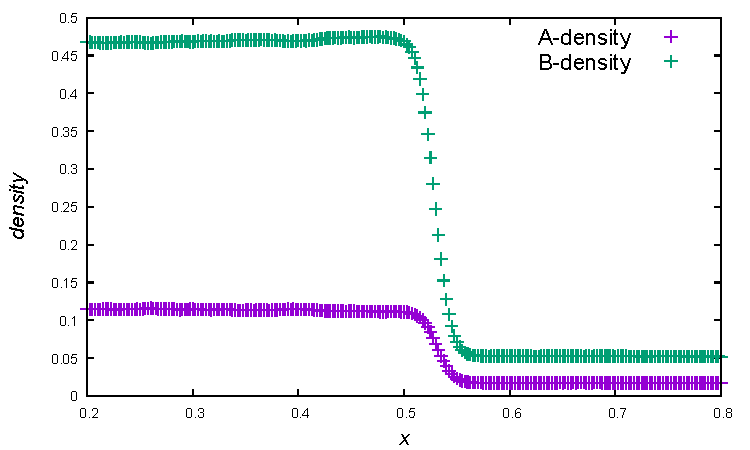
\includegraphics[width=14cm]{fig/lan140493-lbn561971-ran3930-rbn15722/lan140493-lbn561971-ran3930-rbn15722.pdf}
    \end{center}
    \caption{相互作用が対称な二成分LJ系における各粒子の密度の位置依存性}
    \label{fig:lan140493-lbn561971-ran3930-rbn15722}
\end{figure}

\newpage
図\ref{fig:lan140493-lbn561971-ran3930-rbn15722}より、A,Bともに$x:0.2〜0.45$で液体状態を、$x:0.45〜0.55$で気液界面を、$x:0.55〜0.8$で気体状態をとる、気液共存状態が実現されていることが分かる。図\ref{fig:lan140493-lbn561971-ran3930-rbn15722}で得られた密度を式(\ref{eq:gas-liquid-interface-density-profile})を目的関数としLevenberg-Marquardt法により近似したものを図\ref{fig:lan140493-lbn561971-ran3930-rbn15722-fitting}に示す。

\begin{figure}[htbp]
    \begin{center}
        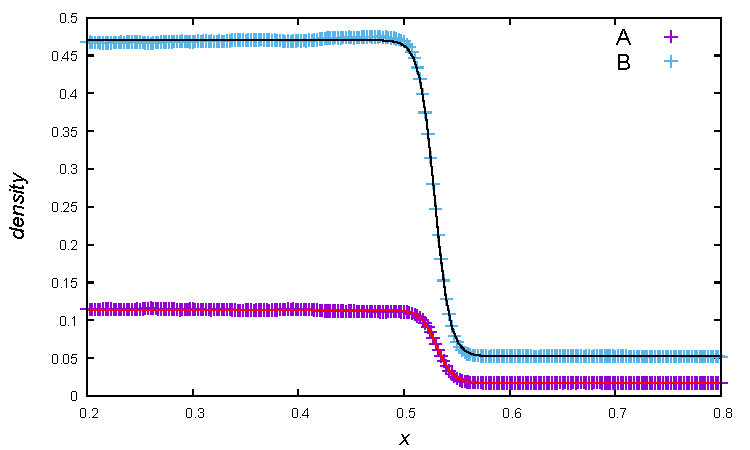
\includegraphics[width=14cm]{fig/lan140493-lbn561971-ran3930-rbn15722/lan140493-lbn561971-ran3930-rbn15722-fitting.pdf}
    \end{center}
    \caption{相互作用が対称な二成分LJ系における各粒子の密度の位置依存性及びその近似}
    \label{fig:lan140493-lbn561971-ran3930-rbn15722-fitting}
\end{figure}

\newpage

図\ref{fig:lan140493-lbn561971-ran3930-rbn15722-fitting}より得られた、気液共存状態におけるA, Bの気相密度$g_A, g_B$、液相密度$l_A, l_B$、$X=g_Al_B-l_Ag_B$を表\ref{table:lan140493-lbn561971-ran3930-rbn15722-fitting}に示す。

\begin{table}[htbp]
    \begin{center}
        \caption{相互作用が対称な二成分LJ系における各粒子の気液密度及び、Xの値}
        \label{table:lan140493-lbn561971-ran3930-rbn15722-fitting}
        \begin{tabular}{c c c c c}
            $g_A$ & $g_B$ & $l_A$ & $l_B$ & $X$ \\
            \hline
            0.01728(8)& 0.0525(2) & 0.11375(7) & 0.4702(1) & 0.00215(4) \\
        \end{tabular}
    \end{center}
\end{table}

表\ref{table:lan140493-lbn561971-ran3930-rbn15722-fitting}に示すように、Aの組成比0.2の時の、$X$の値を導出することが出来る。Aの組成比を0.02〜0.98に0.02刻みで変化させ、上記と同様のプロセスで各組成比における$X$を導出する。図\ref{fig:bi-symmetric}に、Aの組成比とその各組成比における$X$を示す。

\begin{figure}[htbp]
    \begin{center}
        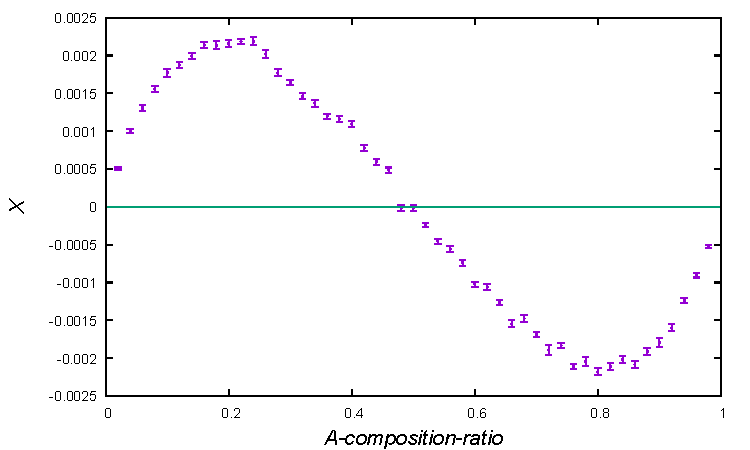
\includegraphics[width=14cm]{fig/bi-symmetric/L100T1.0.pdf}
    \end{center}
    \caption{相互作用が対称な二成分LJ系におけるAの組成比とその各組成比における$X$}
    \label{fig:bi-symmetric}
\end{figure}

\newpage
共沸条件は$X=0$であるから、図\ref{fig:bi-symmetric}より、Aの組成比$\approx0.5$で共沸現象が実現されていることが分かる。

\newpage
\subsection{相互作用が非対称な二成分LJ系における共沸現象の実現} \label{results-subsec:bi-asymmetric-component-azeotrope}
相互作用が非対称な二成分LJ系においても、Aの組成比を0.02〜0.98に0.02刻みで変化させ、\ref{results-subsec:bi-symmetric-component-azeotrope}節と同様のプロセスで各組成比における$X$を導出する。図\ref{fig:bi-asymmetric}に、Aの組成比とその各組成比における$X$を示す。

\begin{figure}[htbp]
    \begin{center}
        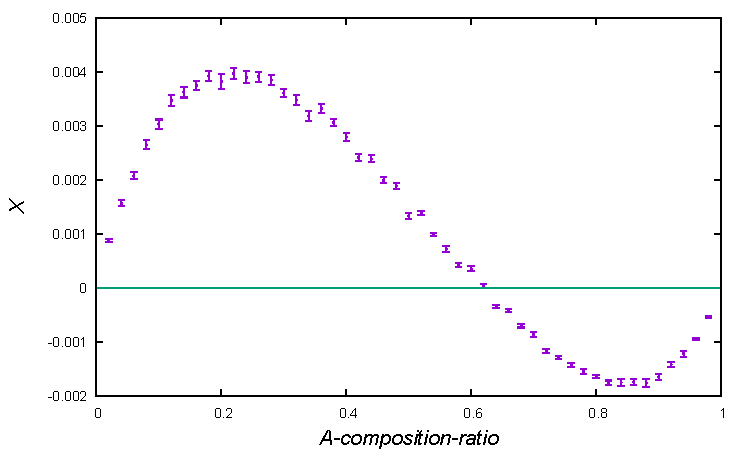
\includegraphics[width=14cm]{fig/bi-asymmetric/L100T1.0E1.05.pdf}
    \end{center}
    \caption{相互作用が非対称な二成分LJ系におけるAの組成比とその各組成比における$X$}
    \label{fig:bi-asymmetric}
\end{figure}

共沸条件は$X=0$であるから、図\ref{fig:bi-asymmetric}よりAの組成比$\neq0.5$で共沸現象が実現されていることが分かる。

\newpage
\section{二成分LJ系におけるポテンシャルパラメタと共沸組成の関係} \label{results-sec:bi-component-potential-parameter-azeotrope-ratio}
\subsection{二成分LJ系における$\sigma$と共沸組成の関係} \label{results-subsec:bi-component-sigma-azeotrope-ratio}
\ref{results-subsec:bi-asymmetric-component-azeotrope}節と同様のプロセスで相互作用が非対称な二成分LJ系におけるBの組成比とその各組成比における$X$の関係を得る。ここで、図\ref{fig:bi-asymmetric}のx軸をBの組成比に置き換えたものを図\ref{fig:bi-asymmetric-b}に示す。

\begin{figure}[htbp]
    \begin{center}
        \includegraphics[width=14cm]{fig/bi-asymmetric-b/L100T1.0E1.05.pdf}
    \end{center}
    \caption{相互作用が非対称な二成分LJ系におけるBの組成比とその各組成比における$X$}
    \label{fig:bi-asymmetric-b}
\end{figure}

\newpage
図\ref{fig:bi-asymmetric-b}の赤く囲まれた部分を抽出し、以下の図\ref{fig:bi-asymmetric-b-part}のようにして、共沸組成を誤差付きで導出する。

\begin{figure}[htbp]
    \begin{center}
        \includegraphics[width=14cm]{fig/bi-asymmetric-b-part/L100T1.0E1.05.pdf}
    \end{center}
    \caption{相互作用が非対称な二成分LJ系における共沸組成近傍のBの組成比と$X$}
    \label{fig:bi-asymmetric-b-part}
\end{figure}

\newpage
図\ref{fig:bi-asymmetric-b-part}のようにして、$\sigma=0.925〜1.2$の各$\sigma$におけるBの共沸組成比を求める。このようにして導出した$\sigma$とその各$\sigma$におけるBの共沸組成比を図\ref{fig:sigma-composition_ratio}に示す。

\begin{figure}[htbp]
    \begin{center}
        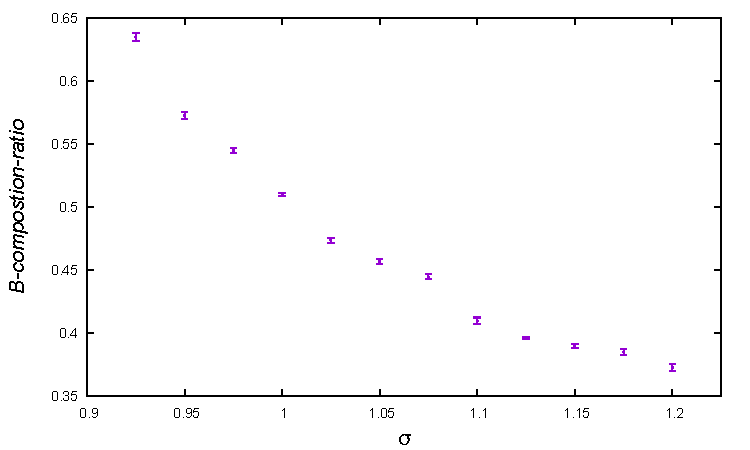
\includegraphics[width=14cm]{fig/sigma-composition_ratio/sigma-composition_ratio.pdf}
    \end{center}
    \caption{二成分LJ系における$\sigma$とBの組成比の関係}
    \label{fig:sigma-composition_ratio}
\end{figure}

図\ref{fig:sigma-composition_ratio}から、$\sigma$を大きくすればするほど、その物質の共沸組成が小さくなることが分かる。

\newpage
\subsection{二成分LJ系における$\epsilon$と共沸組成の関係} \label{results-subsec:bi-component-epsilon-azeotrope-ratio}
\ref{results-subsec:bi-component-sigma-azeotrope-ratio}節と同様のプロセスで、$\epsilon=0.925〜1.3$の各$\epsilon$におけるBの共沸組成比を求める。このようにして導出した$\epsilon$とその各$\epsilon$におけるBの共沸組成比を図\ref{fig:epsilon-composition_ratio}に示す。

\begin{figure}[htbp]
    \begin{center}
        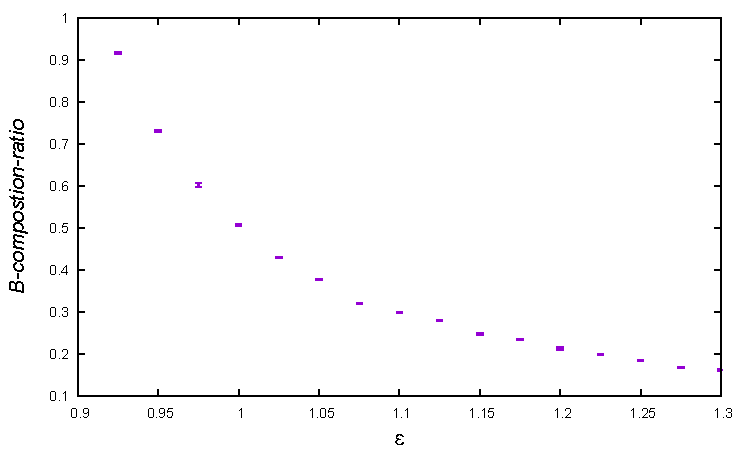
\includegraphics[width=14cm]{fig/epsilon-composition_ratio/epsilon-composition_ratio.pdf}
    \end{center}
    \caption{二成分LJ系における$\epsilon$とBの組成比の関係}
    \label{fig:epsilon-composition_ratio}
\end{figure}

図\ref{fig:epsilon-composition_ratio}から、$\epsilon$を大きくすればするほど、その物質の共沸組成が小さくなることが分かる。


\newpage
\section{相互作用が対称な二成分LJ系への第三成分の添加による目的物質の最高濃度の上昇} \label{results-sec:bi-component-addition-of-3rd-component-highest-purity}
\subsection{第三成分の添加による目的物質の最高濃度の上昇} \label{results-subsec:bi-component-addition-of-3rd-component-highest-purity}
\ref{method-subsec:bi-component-addition-of-3rd-component-highest-purity}節で示したパラメタでMDシミュレーションをLAMMPSで実行して、各粒子の座標を出力する。図\ref{fig:bi-component-addition-of-3rd-component-highest-purity-sample}に、Aの組成比0.396, Bの組成比0.594, Cの組成比0.01の時の最終ステップの粒子のスナップショットを示す。

\begin{figure}[htbp]
    \begin{center}
        
\includegraphics[width=14cm]{fig/sample.jpeg}
    \end{center}
    \caption{対称二成分LJ系に第三成分を添加した系における最終ステップの粒子のスナップショット}
    \label{fig:bi-component-addition-of-3rd-component-highest-purity-sample}
\end{figure}

図\ref{fig:bi-component-addition-of-3rd-component-highest-purity-sample}の出力結果を元に測定された、各位置$x$\,(0.0:最小、1.0:最大において0.2〜0.8の範囲)とその密度の関係を図\ref{fig:lan278176-lbn417263-lcn7025-ran7782-rbn11673-rcn197}に示す。ただし、各粒子の密度は、最後の1000000ステップから1000ステップ刻みに各粒子の位置座標を出力した1000個の結果の平均を取るものとする。

\begin{figure}[htbp]
    \begin{center}
        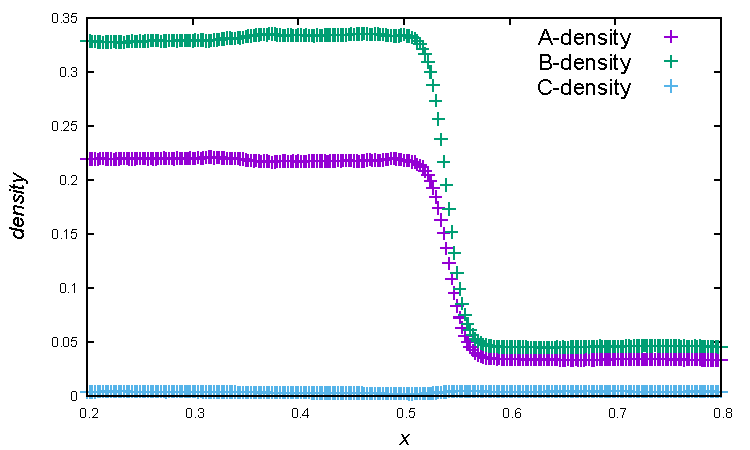
\includegraphics[width=14cm]{fig/lan278176-lbn417263-lcn7025-ran7782-rbn11673-rcn197/lan278176-lbn417263-lcn7025-ran7782-rbn11673-rcn197.pdf}
    \end{center}
    \caption{対称二成分LJ系に第三成分を添加した系における密度の位置依存性}
    \label{fig:lan278176-lbn417263-lcn7025-ran7782-rbn11673-rcn197}
\end{figure}

\newpage
図\ref{fig:lan278176-lbn417263-lcn7025-ran7782-rbn11673-rcn197}より、A,B,C全てにおいて$x:0.2〜0.5$で液体状態を、$x:0.5〜0.55$で気液界面を、$x:0.55〜0.8$で気体状態をとる、気液共存状態が実現されていることが分かる。図\ref{fig:lan278176-lbn417263-lcn7025-ran7782-rbn11673-rcn197}で得られた密度を式(\ref{eq:gas-liquid-interface-density-profile})を目的関数としLevenberg-Marquardt法により近似したものを図\ref{fig:lan278176-lbn417263-lcn7025-ran7782-rbn11673-rcn197-fitting}に示す。

\begin{figure}[htbp]
    \begin{center}
        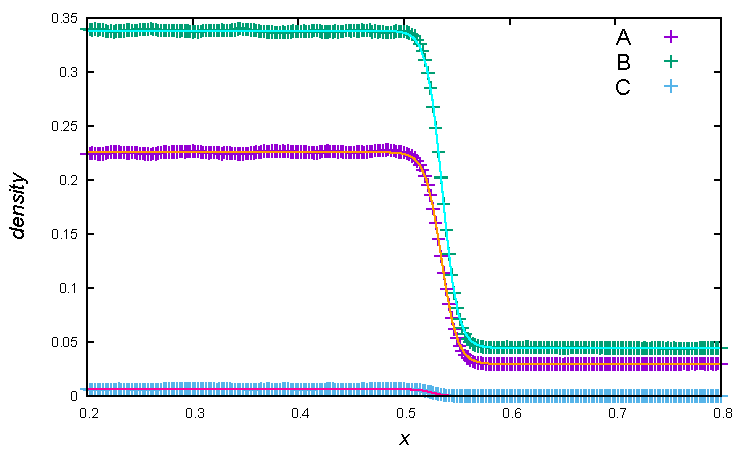
\includegraphics[width=14cm]{fig/lan278176-lbn417263-lcn7025-ran7782-rbn11673-rcn197/lan278176-lbn417263-lcn7025-ran7782-rbn11673-rcn197-fitting.pdf}
    \end{center}
    \caption{対称二成分LJ系に第三成分を添加した系における各粒子の密度の位置依存性及びその近似}
    \label{fig:lan278176-lbn417263-lcn7025-ran7782-rbn11673-rcn197-fitting}
\end{figure}

\newpage

図\ref{fig:lan278176-lbn417263-lcn7025-ran7782-rbn11673-rcn197-fitting}より、気液共存状態におけるA, B, Cの気相密度$g_A, g_B, g_C$、液相密度$l_A, l_B, l_C$の値を基にBの気相, 液相濃度を導出し、各組成においても同様にBの気相, 液相濃度を導出する。また、同様の手法で対称二成分LJ系においても気相, 液相濃度を導出し、Bの液相濃度を横軸に、Bの気相濃度を縦軸に取った図を図\ref{fig:bi-component-addition-of-3rd-component-highest-purity}に示す。

\begin{figure}[htbp]
    \begin{center}
        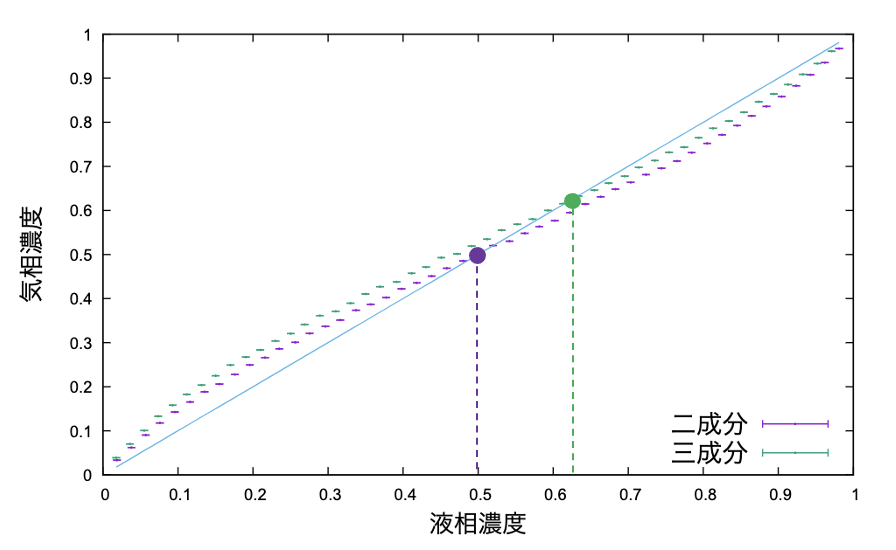
\includegraphics[width=14cm]{fig/highest-purity-difference-E2.0/highest-purity-difference-E2.0.png}
    \end{center}
    \caption{対称二成分LJ系と第三成分を添加した系における目的物質の最高濃度の比較}
    \label{fig:bi-component-addition-of-3rd-component-highest-purity}
\end{figure}

\newpage
図\ref{fig:bi-component-addition-of-3rd-component-highest-purity}に示した対称二成分LJ系と第三成分を添加した系において得られる目的物質Bの最高濃度を表\ref{table:bi-component-addition-of-3rd-component-highest-purity}に示す。

\begin{table}[htbp]
    \begin{center}
        \caption{対称二成分LJ系と第三成分を添加した系において、Bの初期濃度0.1の時に三段で到達する濃度}
        \label{table:bi-component-addition-of-3rd-component-highest-purity}
        \begin{tabular}{c c}
            対称二成分系 & 第三成分を添加した系 \\
            \hline
            0.5 & 0.62806 \\
        \end{tabular}
    \end{center}
\end{table}

表\ref{table:bi-component-addition-of-3rd-component-highest-purity}より、添加物Cを$1.0\%$加えることにより、目的物質Bの最高濃度が約$25.6\%$上がっていることが分かる。

\subsection{第三成分の添加割合と目的物質の最高濃度の関係} \label{results-subsec:bi-component-addition-of-3rd-component-addition-ratio-highest-purity}
\ref{results-subsec:bi-component-addition-of-3rd-component-highest-purity}節と同様の手順で、第三成分の添加割合を$0.0,0.5,1.0,1.5,2.0\%$で変化させた時の目的物質Bの最高濃度を調べる。
図\ref{fig:bi-component-addition-of-3rd-component-addition-ratio-highest-purity}に第三成分の添加割合と目的物質の最高濃度の関係を示す。

\begin{figure}[htbp]
    \begin{center}
        
\includegraphics[width=14cm]{fig/sample.jpeg}
    \end{center}
    \caption{対称二成分LJ系に第三成分を添加した系における第三成分の添加割合と目的物質の最高濃度の関係}
    \label{fig:bi-component-addition-of-3rd-component-addition-ratio-highest-purity}
\end{figure}

図\ref{fig:bi-component-addition-of-3rd-component-addition-ratio-highest-purity}より、第三成分の添加割合を増やせば増やすほど、目的物質Bの最高濃度が上昇していることがわかる。


\section{相互作用が対称な二成分LJ系への第三成分の添加による特定段数で到達する目的物質の濃度の上昇} \label{results-sec:bi-component-addition-of-3rd-component-steps}
\subsection{第三成分の添加による特定段数で到達する目的物質の濃度の上昇} \label{results-subsec:bi-component-addition-of-3rd-component-steps}
目的物質Bの初期濃度0.1の時、対称二成分LJ系において三段で到達する濃度と、第三成分を添加した系において三段で到達する濃度を求める。対称二成分LJ系におけるBの液-気相濃度図とBの初期濃度0.1において三段で到達する濃度を導出する様子を図\ref{fig:bi-component-addition-of-3rd-component-steps-two-comnponent}に、第三成分を添加した系におけるBの液-気相濃度図とBの初期濃度0.1において三段で到達する濃度を導出する様子を図\ref{fig:bi-component-addition-of-3rd-component-steps-three-comnponent}に示す。
尚、それぞれの曲線を5次関数に近似した上で段数の計算を行なった。

\begin{figure}[htbp]
    \begin{center}
        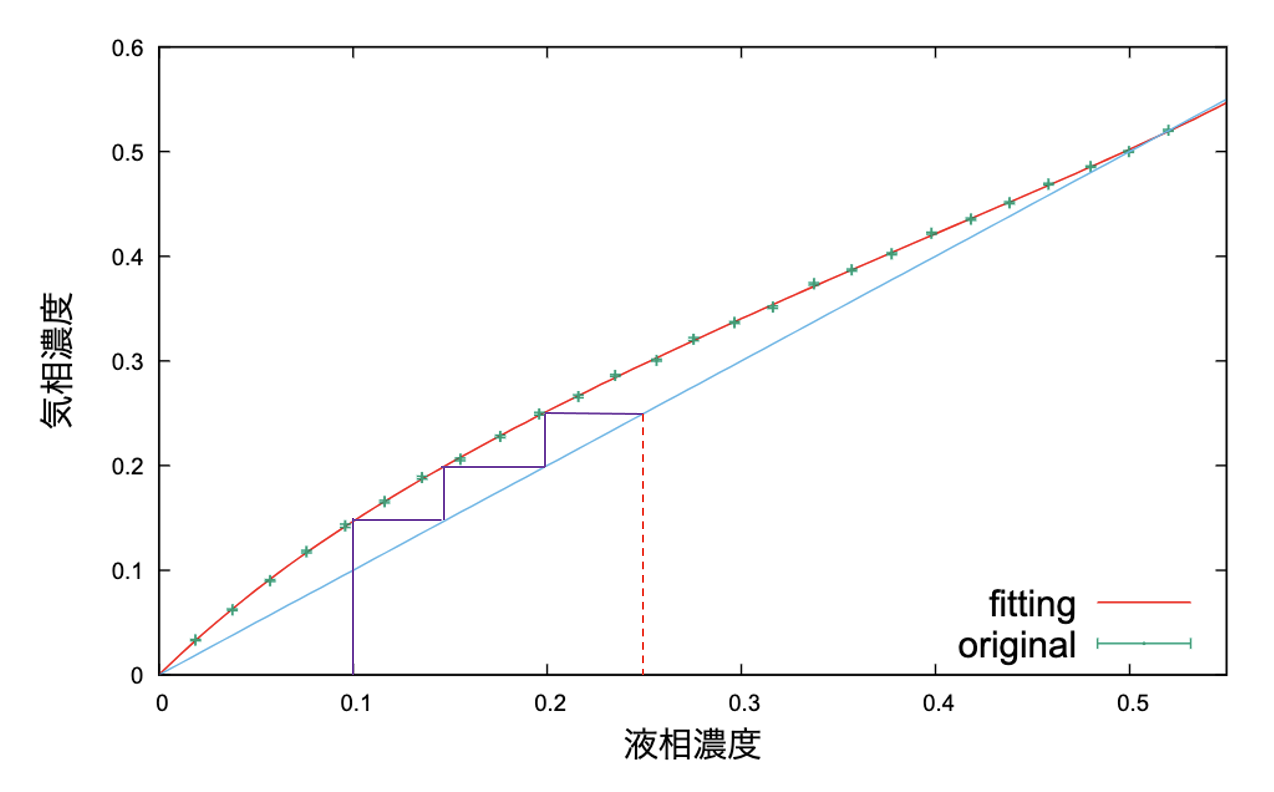
\includegraphics[width=14cm]{fig/steps-difference-E2.0/L100T1.0-part-fitting.png}
    \end{center}
    \caption{対称二成分LJ系において三段で到達する濃度の比較}
    \label{fig:bi-component-addition-of-3rd-component-steps-two-comnponent}
\end{figure}

\begin{figure}[htbp]
    \begin{center}
        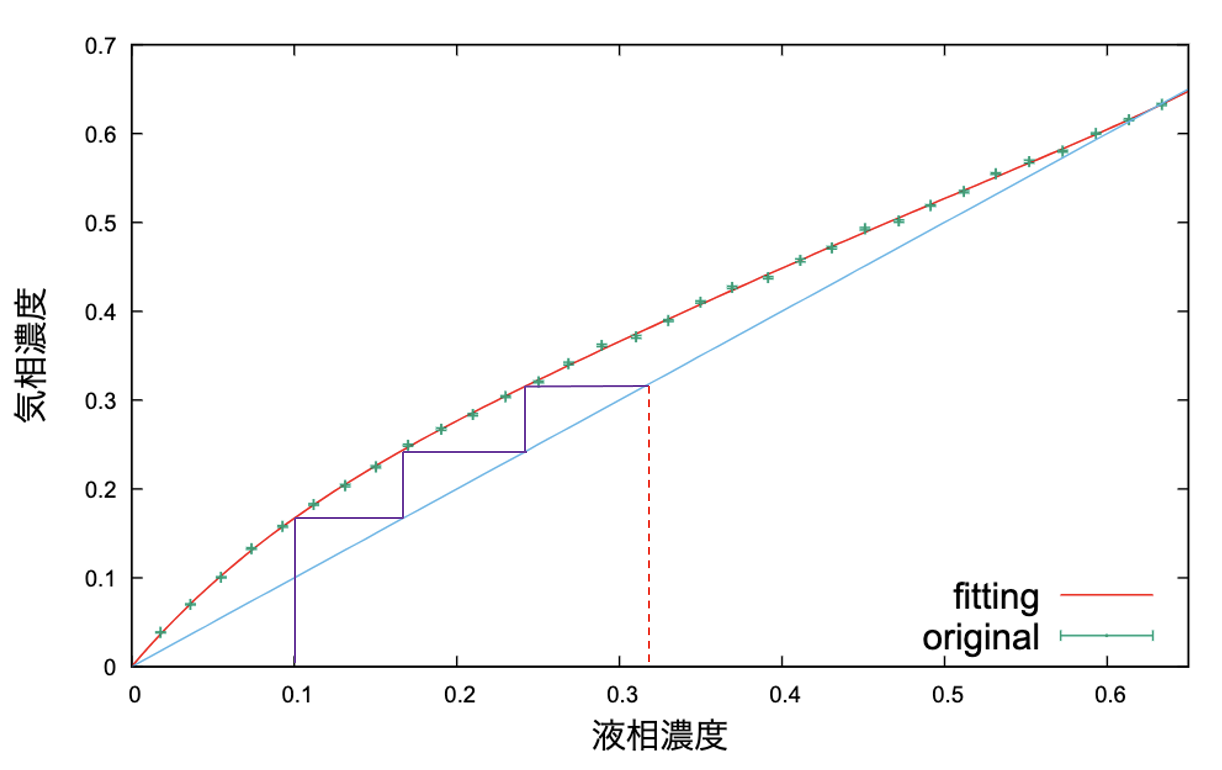
\includegraphics[width=14cm]{fig/steps-difference-E2.0/L100T1.0CN50E2.0CD0.01-part-fitting.png}
    \end{center}
    \caption{第三成分を添加した系において三段で到達する濃度の比較}
    \label{fig:bi-component-addition-of-3rd-component-steps-three-comnponent}
\end{figure}

\newpage
図\ref{fig:bi-component-addition-of-3rd-component-steps-two-comnponent}, 図\ref{fig:bi-component-addition-of-3rd-component-steps-three-comnponent}に示した対称二成分LJ系と第三成分を添加した系において、Bの初期濃度0.1の時に三段で到達する濃度を表\ref{table:bi-component-addition-of-3rd-component-steps}に示す。

\begin{table}[htbp]
    \begin{center}
        \caption{対称二成分LJ系と第三成分を添加した系において、Bの初期濃度0.1の時に三段で到達する濃度}
        \label{table:bi-component-addition-of-3rd-component-steps}
        \begin{tabular}{c c}
            対称二成分系 & 第三成分を添加した系 \\
            \hline
            0.25089 & 0.31701 \\
        \end{tabular}
    \end{center}
\end{table}

表\ref{table:bi-component-addition-of-3rd-component-steps}より、添加物Cを$1.0\%$加えることにより、三段で到達する目的物質Bの濃度が約$26.4\%$上がっていることが分かる。


\subsection{第三成分の添加割合と特定段数で到達する目的物質の濃度の関係} \label{results-subsec:bi-component-addition-of-3rd-component-addition-ratio-steps}
\ref{results-subsec:bi-component-addition-of-3rd-component-steps}と同様の手順で、第三成分の添加割合を$0.0,0.5,1.0,1.5,2.0\%$に変化させた時の三段で到達する目的物質Bの濃度を調べる。
図\ref{fig:bi-component-addition-of-3rd-component-addition-ratio-steps}に第三成分の添加割合と三段で到達する目的物質の濃度を示す。

\begin{figure}[htbp]
    \begin{center}
        
\includegraphics[width=14cm]{fig/sample.jpeg}
    \end{center}
    \caption{対称二成分LJ系に第三成分を添加した系における第三成分の添加割合と三段で到達する目的物質Bの濃度の関係}
    \label{fig:bi-component-addition-of-3rd-component-addition-ratio-steps}
\end{figure}

\newpage
図\ref{fig:bi-component-addition-of-3rd-component-addition-ratio-steps}より、第三成分の添加割合を増やせば増やすほど、三段で到達する目的物質Bの濃度が上昇することが分かる。


\chapter{結論及び考察} \label{chap:summary}
我々は分子動力学(Molecular Dynamics, MD)法\cite{molecular-dynamics}により、一つのシミュレーションボックスで気液共存状態を実現することで、より安定で精度が高く、並列計算に向いた手法で共沸現象を実現することを第一の目的と、既存の手法で困難であった第三成分の添加による目的物質の最高濃度を上げること、特定段数で到達する目的物質の濃度を上げることを第二の目的としたが、これは共に達成された。\\
まず、一つのシミュレーションボックスで共沸現象を実現したが、これは共沸現象の研究へ新たなアプローチを提案するものであり、実在する系を正確にモデリング出来れば、実在する系についても正確で早い共沸現象の実現をサポートするものである。\\
続いて、第三成分の添加による目的物質の最高濃度を上げること、特定段数で到達する目的物質の濃度を上げることに成功したが、これはどのような第三成分を添加することにより、どれだけ目的物質の最高濃度や段数を変更できるかをよりミクロに調べる方法として非常に有用である。

% 考察は、「研究の背景」及び「目的」において提起した問題に正しく答えるようにする。得られた結果は満足すべきものだったか?不満があるならその理由はなにか?解決できそうなのか?また、「大きい理由」にも言及する。本研究によりどのような課題が見つかったかを書き、この分野における「研究の流れ」においてのような位置づけにあるかを説明した上で、今後、どのような発展の方向があるかについて書く。

\chapter*{謝辞}
まず、研究を進める上で、基礎的な部分から多くの指導をしていただいた渡辺宙志准教授には大変感謝しております。
研究のみならず、就職活動などにも気にかけ、全面的にサポートしていただき、心より御礼申し上げます。
また、同じ研究室に所属していた藤田くん、四辻くん、佐藤くんは、同期として切磋琢磨しながら研究を進めることが出来ましたこと、深く感謝致します。
最後に、研究のみならず、学生生活を様々な面でサポートしてくださった両親に深く感謝致します。

\appendix
\chapter{ohtakaにおけるジョブの扱い}
\lstinputlisting[caption = 49本のシミュレーションを並列実行するジョブスクリプト, label = prog:job, basicstyle=\footnotesize\ttfamily, breaklines=true]{src/L100T1.0CN50E1.05CD0.01-job.sh}

\chapter{ソースコード}
\lstinputlisting[caption = 三成分系の粒子生成用スクリプト, label=prog:generate_atoms,   basicstyle=\footnotesize\ttfamily, breaklines=true]{src/generate_atoms.py}
\lstinputlisting[caption = 三成分系のdump出力用スクリプト, label=prog:generate_in.melt,   basicstyle=\footnotesize\ttfamily, breaklines=true]{src/generate_in.melt.py}
\lstinputlisting[caption = 三成分系の共沸点出力用スクリプト, label=prog:generate_azeotrope,   basicstyle=\footnotesize\ttfamily, breaklines=true]{src/generate_azeotrope.py}

\bibliographystyle{junsrt}
\bibliography{reference}

\end{document}
